%%============================================================
%% ENTREGABLE — TE3001B Fundamentación de Robótica
%% Teleoperación con Sensado de Fuerza: xArm Lite 6 (Maestro-Esclavo)
%% Formato IEEE Transactions — Plantilla para Alumnos
%% Prof. Alberto Muñoz — Computational Robotics Lab
%% Tecnológico de Monterrey — 2026
%% ============================================================
\documentclass[journal,10pt,twoside]{IEEEtran}

%% ── Paquetes base ────────────────────────────────────────────
\usepackage[utf8]{inputenc}
\usepackage[T1]{fontenc}
\usepackage[spanish,es-nodecimaldot]{babel}
\usepackage{amsmath,amssymb,bm}
\usepackage{graphicx}
\usepackage{xcolor}
\usepackage{hyperref}
\usepackage{booktabs}
\usepackage{multirow}
\usepackage{array}
\usepackage{colortbl}
\usepackage{caption}
\usepackage{subcaption}
\usepackage{listings}
\usepackage{tcolorbox}
\usepackage{enumitem}
\usepackage{tikz}
\usepackage{pgfplots}
\usepackage{url}
\usepackage{float}
\pgfplotsset{compat=1.18}
\usetikzlibrary{arrows.meta,shapes,positioning,calc,backgrounds}
\tcbuselibrary{breakable,skins}

\hypersetup{colorlinks=true, linkcolor=tec_blue, urlcolor=tec_blue,
            citecolor=tec_blue}

%% ── Colores institucionales ──────────────────────────────────
\definecolor{tec_blue}{RGB}{0,68,124}
\definecolor{tec_lightblue}{RGB}{0,140,200}
\definecolor{tec_red}{RGB}{190,30,45}
\definecolor{tec_gray}{RGB}{100,100,100}
\definecolor{code_bg}{RGB}{245,247,250}
\definecolor{code_kw}{RGB}{0,100,180}
\definecolor{code_str}{RGB}{180,50,20}
\definecolor{code_cmt}{RGB}{80,140,80}
\definecolor{box_todo}{RGB}{255,243,205}
\definecolor{box_todo_border}{RGB}{200,140,0}
\definecolor{box_rubric}{RGB}{232,245,233}
\definecolor{box_rubric_border}{RGB}{67,160,71}
\definecolor{box_theory}{RGB}{227,242,253}
\definecolor{box_theory_border}{RGB}{25,118,210}

%% ── Cajas de tcolorbox ───────────────────────────────────────
\newtcolorbox{todobox}[1][Completar]{
  colback=box_todo, colframe=box_todo_border,
  title={\textbf{$\triangleright$ #1}},
  fonttitle=\bfseries\color{tec_gray},
  breakable, enhanced, left=4pt, right=4pt
}
\newtcolorbox{rubricbox}[1][Rúbrica]{
  colback=box_rubric, colframe=box_rubric_border,
  title={\textbf{\checkmark\ Criterio de Evaluación — #1}},
  fonttitle=\bfseries\small\color{box_rubric_border},
  breakable, enhanced, left=4pt, right=4pt
}
\newtcolorbox{theorybox}[1][Marco Teórico]{
  colback=box_theory, colframe=box_theory_border,
  title={\textbf{(i) Contexto: #1}},
  fonttitle=\bfseries\small\color{tec_blue},
  breakable, enhanced, left=4pt, right=4pt
}

%% ── Estilo de código ─────────────────────────────────────────
\lstdefinestyle{python}{
  language=Python,
  backgroundcolor=\color{code_bg},
  basicstyle=\ttfamily\scriptsize,
  keywordstyle=\color{code_kw}\bfseries,
  stringstyle=\color{code_str},
  commentstyle=\color{code_cmt}\itshape,
  numbers=left, numberstyle=\tiny\color{tec_gray},
  numbersep=6pt, frame=single, tabsize=4,
  showstringspaces=false, breaklines=true,
  morekeywords={import,from,as,def,class,return,True,False,None,self},
  literate={á}{{\'{a}}}1 {é}{{\'{e}}}1 {í}{{\'{i}}}1
           {ó}{{\'{o}}}1 {ú}{{\'{u}}}1 {ñ}{{\~{n}}}1,
}
\lstset{style=python}

%% ── Macros de ayuda ──────────────────────────────────────────
\newcommand{\answerline}[1][3cm]{\underline{\hspace{#1}}}
\newcommand{\pts}[1]{\textbf{\color{tec_red}[#1 pts]}}
\newcommand{\TODO}[1]{\begin{todobox}[Respuesta del equipo]
  \textit{#1}
\end{todobox}}
\newcommand{\FIGURE}[1]{\begin{todobox}[Insertar figura]
  \centering
  \begin{tikzpicture}
    \draw[tec_gray, dashed, line width=1pt] (0,0) rectangle (8,4);
    \node[tec_gray, font=\small] at (4,2) {#1};
  \end{tikzpicture}
\end{todobox}}

%% ── Metadatos del artículo ───────────────────────────────────
\begin{document}

\title{Teleoperación con Sensado de Fuerza Física\\
  entre dos xArm Lite 6:\\
  Diseño, Implementación y Evaluación Experimental}

\author{%
  \IEEEauthorblockN{%
    Ángel Domínguez Faraco \IEEEauthorrefmark{1},\;
    Pablo Díaz Aguilar\IEEEauthorrefmark{1},\;
    José Omar Cavazos González\IEEEauthorrefmark{1},\;
    Lucas Tavares Quintela Blanc \IEEEauthorrefmark{1},\;
    Nabor Sebastian Toro García\IEEEauthorrefmark{1}
  }\\
  \IEEEauthorblockA{%
    \IEEEauthorrefmark{1}%
    Computational Robotics Lab, Tecnológico de Monterrey,
    Monterrey, N.L., México\\
    \texttt{\{A00835367, A00836765, A00840617, A01028428, A01831998\}@tec.mx}
  }
}

\maketitle

%% ── Abstract ─────────────────────────────────────────────────
\begin{abstract}
La necesidad de manipular objetos en entornos donde la presencia humana es imposible, costosa o peligrosa ha impulsado el desarrollo de sistemas de teleoperación avanzados. A diferencia de la teleoperación convencional basada únicamente en retroalimentación visual, la integración de retroalimentación háptica permite al operador recuperar la sensación de presencia física en el entorno remoto. Este proyecto se motiva por la capacidad de cerrar el lazo de fuerza entre dos manipuladores xArm Lite 6, permitiendo que la interacción mecánica en el \textbf{Esclavo} sea percibida táctilmente en el \textbf{Maestro}.

Esta tecnología es crítica en sectores donde la precisión y el sentido del tacto son determinantes para el éxito de la misión. Por ejemplo, en la cirugía robótica, el uso de sistemas bilaterales permite a los cirujanos percibir la elasticidad y resistencia de los tejidos internos durante procedimientos mínimamente invasivos, lo cual reduce significativamente el riesgo de trauma accidental por exceso de presión [1].

Asimismo, en el ámbito del mantenimiento industrial y aeroespacial, la teleoperación con sensado de fuerza es indispensable para la manipulación de materiales peligrosos o la reparación de satélites en órbita. En estas situaciones, el operador requiere ``sentir'' si un componente ha encajado correctamente en su posición o si un tornillo ha alcanzado el torque adecuado, superando las limitaciones de profundidad que presentan las cámaras 2D convencionales [2]. El uso del protocolo ROS 2 y sensores de carga como el HX711 en este proyecto busca emular estas capacidades industriales mediante una arquitectura de baja latencia y alta fidelidad.

\end{abstract}

\begin{IEEEkeywords}
  teleoperación, sensado de fuerza, xArm Lite 6, control de impedancia,
  retroalimentación háptica, arquitectura maestro-esclavo, ROS2 (Robot Operating System)
\end{IEEEkeywords}

%% ============================================================
\section{Introducción}
%% ============================================================

\IEEEPARstart{L}{a} teleoperación con retroalimentación de fuerza
constituye un paradigma fundamental en robótica cuando se requiere que
un operador humano interactúe con entornos remotos o peligrosos sin
presencia física~\cite{murray1994}. El xArm Lite 6, desarrollado por
UFACTORY~\cite{xarm_github}, es un manipulador de 6 grados de libertad
(DOF) con capacidad de control de torque que lo hace idóneo para experimentos
de sensado de fuerza por torque articular.

\begin{theorybox}[Motivación]
  El reto central de este proyecto es cerrar el lazo de fuerza entre
  dos brazos robóticos: el robot \textbf{Maestro}, operado por el humano,
  y el robot \textbf{Esclavo}, que interactúa con el entorno.
  La fuerza de contacto estimada en el esclavo debe reflejarse como
  torque en las articulaciones del maestro, creando la sensación
  háptica que guía al operador.
\end{theorybox}

\subsection{Contexto y Motivación}

La teleoperación con retroalimentación de fuerza ha adquirido
importancia creciente en aplicaciones donde la presencia física del
operador es imposible, costosa o peligrosa~\cite{niemeyer2008}.
Los sistemas bilaterales —aquellos que transmiten información tanto
del operador hacia el robot esclavo como en sentido inverso—
incorporan un canal de retorno de fuerza que permite percibir las
interacciones mecánicas del robot remoto con su entorno,
transformando la teleoperación en una experiencia táctil con
presencia comparable a la manipulación directa~\cite{murray1994}.

En el ámbito médico, la cirugía robótica mínimamente invasiva
representa una de las aplicaciones más exigentes de esta tecnología.
Los sistemas quirúrgicos actuales operan de forma unilateral,
privando al cirujano de la sensación de resistencia y elasticidad
del tejido; la integración de retroalimentación de fuerza permitiría
detectar presiones excesivas sobre estructuras anatómicas sensibles,
reduciendo el riesgo de trauma accidental por exceso de
fuerza~\cite{thompson2001}.

En el ámbito industrial y aeroespacial, tareas de ensamblaje de
precisión como la inserción de piezas con tolerancias reducidas
(\textit{peg-in-hole}) requieren que el operador detecte el instante
en que un componente ha alcanzado su posición correcta.
La retroalimentación háptica sustituye la percepción táctil directa
que se pierde en la operación remota, permitiendo al operador
«sentir» si la inserción fue exitosa o si se está ejerciendo una
fuerza excesiva sobre el entorno~\cite{siciliano2009}.

\medskip
\noindent\rule{\linewidth}{0.4pt}
\medskip

\textbf{Referencias del contexto}
\begin{enumerate}[label={[\arabic*]}]
  \item A. M. Okamura, ``Methods for haptic feedback in teleoperated robot-assisted surgery,'' \textit{Industrial Robot: An International Journal}, vol. 31, no. 6, pp. 499--508, 2004.
  \item R. J. Adams and B. Hannaford, ``Stable haptic interaction with virtual environments,'' \textit{IEEE Transactions on Robotics and Automation}, vol. 15, no. 3, pp. 465--474, 1999.
  \item UFACTORY, ``xArm Lite 6 User Manual and Developer Guide,'' v2.1, 2023. [En línea]. Disponible en: \url{https://www.ufactory.cc/support/}
\end{enumerate}

\subsection{Contribuciones del Trabajo}

Las contribuciones específicas de este trabajo son las siguientes:
\begin{itemize}
  \item \textbf{Arquitectura maestro-esclavo sobre ROS~2:} diseño e
        implementación de un sistema de teleoperación articular a
        30~Hz entre dos xArm Lite~6, usando los namespaces
        \texttt{/ufactory} (maestro) y \texttt{/ufactory2} (esclavo)
        sobre el stack oficial \texttt{xarm\_ros2}.
  \item \textbf{Canal de sensado de fuerza externo de bajo costo:}
        integración de una celda de carga HX711 con un
        microcontrolador ESP32 mediante firmware micro-ROS, que
        publica la fuerza medida en el tópico ROS~2
        \texttt{/load\_cell\_weight} como alternativa accesible
        al sensor F/T dedicado de muñeca.
  \item \textbf{Mecanismo de paro de emergencia por umbral de fuerza:}
        implementación de un E-Stop que coloca ambos brazos en
        \texttt{state=4} al superar el umbral de colisión configurado,
        protegiendo al operador y al entorno físico ante contactos
        no controlados.
  \item \textbf{Suavizado adaptativo de movimiento:} aplicación de
        una media móvil sobre las últimas cuatro posturas articulares
        y un filtro exponencial de primer orden sobre la velocidad
        estimada ($\alpha{=}0.3$), reduciendo el jitter transmitido
        del maestro al esclavo sin incrementar significativamente
        la latencia del lazo.
  \item \textbf{Validación experimental con tarea peg-in-hole:}
        demostración del sistema en operación con hardware físico,
        incluyendo eventos de contacto controlados monitoreados
        mediante el canal de fuerza en tiempo real.
\end{itemize}

\subsection{Estructura del Artículo}
El resto de este artículo se organiza como sigue:
la Sección~\ref{sec:background} presenta los fundamentos teóricos;
la Sección~\ref{sec:architecture} describe la arquitectura del sistema;
la Sección~\ref{sec:force} detalla la estrategia de sensado de fuerza;
la Sección~\ref{sec:control} expone el esquema de control;
la Sección~\ref{sec:implementation} documenta la implementación con xArm SDK;
la Sección~\ref{sec:experiments} reporta los resultados experimentales;
la Sección~\ref{sec:discussion} discute los hallazgos;
y la Sección~\ref{sec:conclusions} concluye el trabajo.

%% ============================================================
\section{Marco Teórico}
\label{sec:background}
%% ============================================================

\subsection{Cinemática y Jacobiano del xArm Lite 6}

El xArm Lite 6 es un manipulador de $n=6$ DOF con articulaciones
rotacionales. Su cinemática directa se describe mediante la convención
Denavit-Hartenberg (DH) o Product of Exponentials (PoE).

\begin{theorybox}[Jacobiano Geométrico]
  El Jacobiano $\bm{J}(\bm{q}) \in \mathbb{R}^{6\times6}$ mapea
  velocidades articulares a velocidades cartesianas del efector final:
  \[
    \begin{pmatrix} \bm{v} \\ \bm{\omega} \end{pmatrix} = \bm{J}(\bm{q})\,\dot{\bm{q}}
  \]
  Su transpuesta mapea fuerzas/torques cartesianos a torques articulares:
  \[
    \bm{\tau} = \bm{J}^\top(\bm{q})\,\bm{F}_{ext}
  \]
  Esta relación es la base del \emph{torque-based force sensing}.
\end{theorybox}

\subsubsection*{Pregunta~T1 \pts{8}}
\begin{enumerate}[label=(\alph*)]
  \item Expliquen la diferencia entre el \textbf{Jacobiano analítico}
        y el \textbf{Jacobiano geométrico} para el xArm Lite 6.
        ¿Cuál utilizan en su implementación y por qué?
  \item Identifiquen y describan \textbf{dos configuraciones singulares}
        del xArm Lite 6 a partir de su geometría DH. ¿Qué ocurre con la
        estimación de fuerza $\hat{\bm{F}} = (\bm{J}^\top)^+\bm{\tau}$
        cerca de esas singularidades?
  \item ¿Cómo detectan programáticamente que el robot está cerca de
        una singularidad? Escriban la condición en términos del
        número de condición $\kappa(\bm{J})$.
\end{enumerate}
\textbf{Respuesta T1}

\begin{enumerate}[label=(\alph*)]
  \item \textbf{Jacobiano Analítico vs. Geométrico:} El Jacobiano geométrico ($\bm{J}$) relaciona velocidades articulares con velocidades lineales y angulares del efector final basándose en la geometría del robot. El analítico usa derivadas de una parametrización de orientación (como ángulos de Euler). En nuestra implementación usamos el \textbf{geométrico} porque su transpuesta mapea directamente fuerzas cartesianas a torques articulares:
  \
  \
  $\bm{\tau} = \bm{J}^{\top} \bm{F}_{ext}$,
  \
  \
  que es la base de la estimación de fuerza.

  \item \textbf{Configuraciones Singulares:} Dos singularidades comunes en el xArm Lite 6 son:
  \begin{enumerate}
    \item \textbf{Singularidad de codo:} cuando el brazo está totalmente extendido.
    \item \textbf{Singularidad de muñeca:} cuando las articulaciones de la muñeca se alinean.
  \end{enumerate}
  Cerca de estas configuraciones, la estimación
  \
  \
  $\hat{\bm{F}} = (\bm{J}^{\top})^{+} \bm{\tau}$
  \
  \
  falla porque el Jacobiano pierde rango y los valores de fuerza calculados tienden al infinito o se vuelven extremadamente ruidosos.

  \item \textbf{Detección Programática:} Se utiliza el número de condición $\kappa(\bm{J})$. Un valor
  \
  \
  $\kappa(\bm{J}) \gg 1$
  \
  \
  indica que el robot está cerca de una singularidad y el control debe saturar o detenerse.
\end{enumerate}

\subsection{Dinámica del Manipulador}

La dinámica de un robot rígido de $n$ DOF se expresa como:
\begin{equation}
  \bm{M}(\bm{q})\ddot{\bm{q}} + \bm{C}(\bm{q},\dot{\bm{q}})\dot{\bm{q}}
  + \bm{g}(\bm{q}) = \bm{\tau} - \bm{J}^\top\bm{F}_{ext}
  \label{eq:dynamics}
\end{equation}
donde $\bm{M}$ es la matriz de inercia, $\bm{C}$ la matriz de
Coriolis/centrífuga y $\bm{g}$ el vector gravitacional.

\subsubsection*{Pregunta~T2 \pts{10}}
\begin{enumerate}[label=(\alph*)]
  \item Partiendo de la Ec.~\eqref{eq:dynamics}, \textbf{deriven} la
        ley de control de par calculado (Computed Torque Control, CTC)
        y demuestren que produce la dinámica de error lineal:
        \[
          \ddot{\bm{e}} + K_v\dot{\bm{e}} + K_p\bm{e} = \bm{0}
        \]
        ¿Qué condiciones sobre $K_p$ y $K_v$ garantizan
        estabilidad asintótica global?
  \item Para el xArm Lite 6 operando en modo \texttt{SERVO} de
        la SDK, el bucle de control interno trabaja a \answerline{1.5cm}~Hz.
        Expliquen cómo esto limita la elección de $K_p$ y $K_v$.
  \item Expresen los polos del sistema cerrado en términos de
        $\omega_n$ (frecuencia natural) y $\zeta$ (amortiguamiento).
        ¿Qué valor de $\zeta$ usaron y por qué?
\end{enumerate}
\textbf{Respuesta T2}

\begin{enumerate}[label=(\alph*)]
  \item \textbf{Ley de Control CTC:} Partiendo de la dinámica
  \
  \
  $\bm{M}(\bm{q})\ddot{\bm{q}} + \bm{C}(\bm{q},\dot{\bm{q}})\dot{\bm{q}} + \bm{g}(\bm{q}) = \bm{\tau}$,
  \
  \
  la ley de control es
  \
  \
  $\bm{\tau} = \bm{M}(\bm{q})[\ddot{\bm{q}}_d + K_v\dot{\bm{e}} + K_p\bm{e}] + \hat{\bm{C}}\dot{\bm{q}} + \hat{\bm{g}}$.
  \
  \
  Esto cancela la dinámica no lineal y produce la dinámica de error lineal
  \
  \
  $\ddot{\bm{e}} + K_v\dot{\bm{e}} + K_p\bm{e} = \bm{0}$.
  \
  \
  Para estabilidad, $K_p$ y $K_v$ deben ser matrices definidas positivas.

  \item \textbf{Limitaciones de la SDK:} La frecuencia de 1.5 kHz (o los 50 Hz configurados en su código de ROS 2) limita la magnitud de las ganancias. Ganancias muy altas con una tasa de muestreo baja introducen ruido de cuantización y aliasing, causando vibraciones mecánicas.
\end{enumerate}
\subsection{Control de Impedancia}

El control de impedancia~\cite{hogan1985} modela el efector final como
un sistema masa-resorte-amortiguador virtual:
\begin{equation}
  \bm{F}_{ctrl} = \bm{K}_d(\bm{x}_d - \bm{x})
                + \bm{B}_d(\dot{\bm{x}}_d - \dot{\bm{x}})
                + \bm{M}_d(\ddot{\bm{x}}_d - \ddot{\bm{x}})
  \label{eq:impedance}
\end{equation}

\subsubsection*{Pregunta~T3 \pts{8}}
\begin{enumerate}[label=(\alph*)]
  \item Para la Ec.~\eqref{eq:impedance}, analicen el efecto de
        aumentar $\bm{K}_d$ en: (i) la sensación háptica del operador,
        (ii) la estabilidad con retardo $T_d$, (iii) la velocidad
        de respuesta ante contacto.
  \item Dado un retardo de red $T_d = 20$~ms medido en su laboratorio,
        calculen la rigidez virtual máxima $K_{d,max}$ que garantiza
        estabilidad usando el criterio de pasividad de Colgate~\cite{colgate1993}:
        \[
          K_{d,max} < \frac{\pi}{2\,T_d\,\omega_c}
        \]
        donde $\omega_c$ es el ancho de banda del controlador interno
        del xArm. Justifiquen el valor de $\omega_c$ que usan.
  \item ¿Usaron impedancia en espacio articular o cartesiano?
        Justifiquen su elección para la tarea de teleoperación.
\end{enumerate}
\TODO{\item[(a)] Al aumentar \(K_d\), la sensación háptica se vuelve más rígida y el contacto se siente más fuerte. También mejora la rapidez de respuesta ante contacto. Sin embargo, con retardo \(T_d\), un \(K_d\) grande reduce la estabilidad y puede causar oscilaciones o vibraciones.

\item[(b)] Usando el criterio de Colgate,

\[
K_{d,\max} < \frac{\pi}{2T_d\omega_c}
\]

con \(T_d = 20~\text{ms} = 0.02~\text{s}\). Si se toma un valor razonable de \(\omega_c = 20~\text{rad/s}\), entonces

\[
K_{d,\max} < \frac{\pi}{2(0.02)(20)} = \frac{\pi}{0.8} \approx 3.93
\]

Por lo tanto,

\[
\boxed{K_{d,\max} \approx 3.9}
\]

\item[(c)] Se prefiere impedancia en \textbf{espacio cartesiano}, porque en teleoperación interesa más controlar cómo se comporta el efector final frente al entorno. Así, el movimiento y el contacto se vuelven más intuitivos para el operador.}

%% ============================================================
\section{Arquitectura del Sistema}
\label{sec:architecture}
%% ============================================================

\subsection{Visión General}

El sistema completo consta de dos xArm Lite 6 conectados a sus
respectivas computadoras de control mediante cable Ethernet, y
comunicados entre sí mediante una red LAN o Wi-Fi.

\subsubsection*{Pregunta~A1 \pts{10}}
\begin{enumerate}[label=(\alph*)]
  \item Elaboren un \textbf{diagrama de bloques} completo del sistema
        maestro-esclavo que incluya: xArm Maestro, PC Maestro,
        protocolo de comunicación, PC Esclavo, xArm Esclavo,
        sensor/estimador de fuerza, y lazo de retroalimentación háptica.
        Indiquen las señales que fluyen entre cada bloque con sus
        dimensiones (e.g., $\bm{q}\in\mathbb{R}^6$, $\bm{F}\in\mathbb{R}^3$).
  \item Describan el \textbf{flujo de datos} en un ciclo de control:
        ¿qué señales se leen del robot Maestro? ¿qué se envía al Esclavo?
        ¿qué se retroalimenta al Maestro?
  \item ¿Cuál es la frecuencia de actualización de su lazo de control?
        Justifiquen por qué eligieron esa frecuencia en relación con
        las capacidades del xArm SDK (\texttt{set\_servo\_angle} vs.
        \texttt{set\_position}).
\end{enumerate}

\begin{figure}[H]
  \centering
  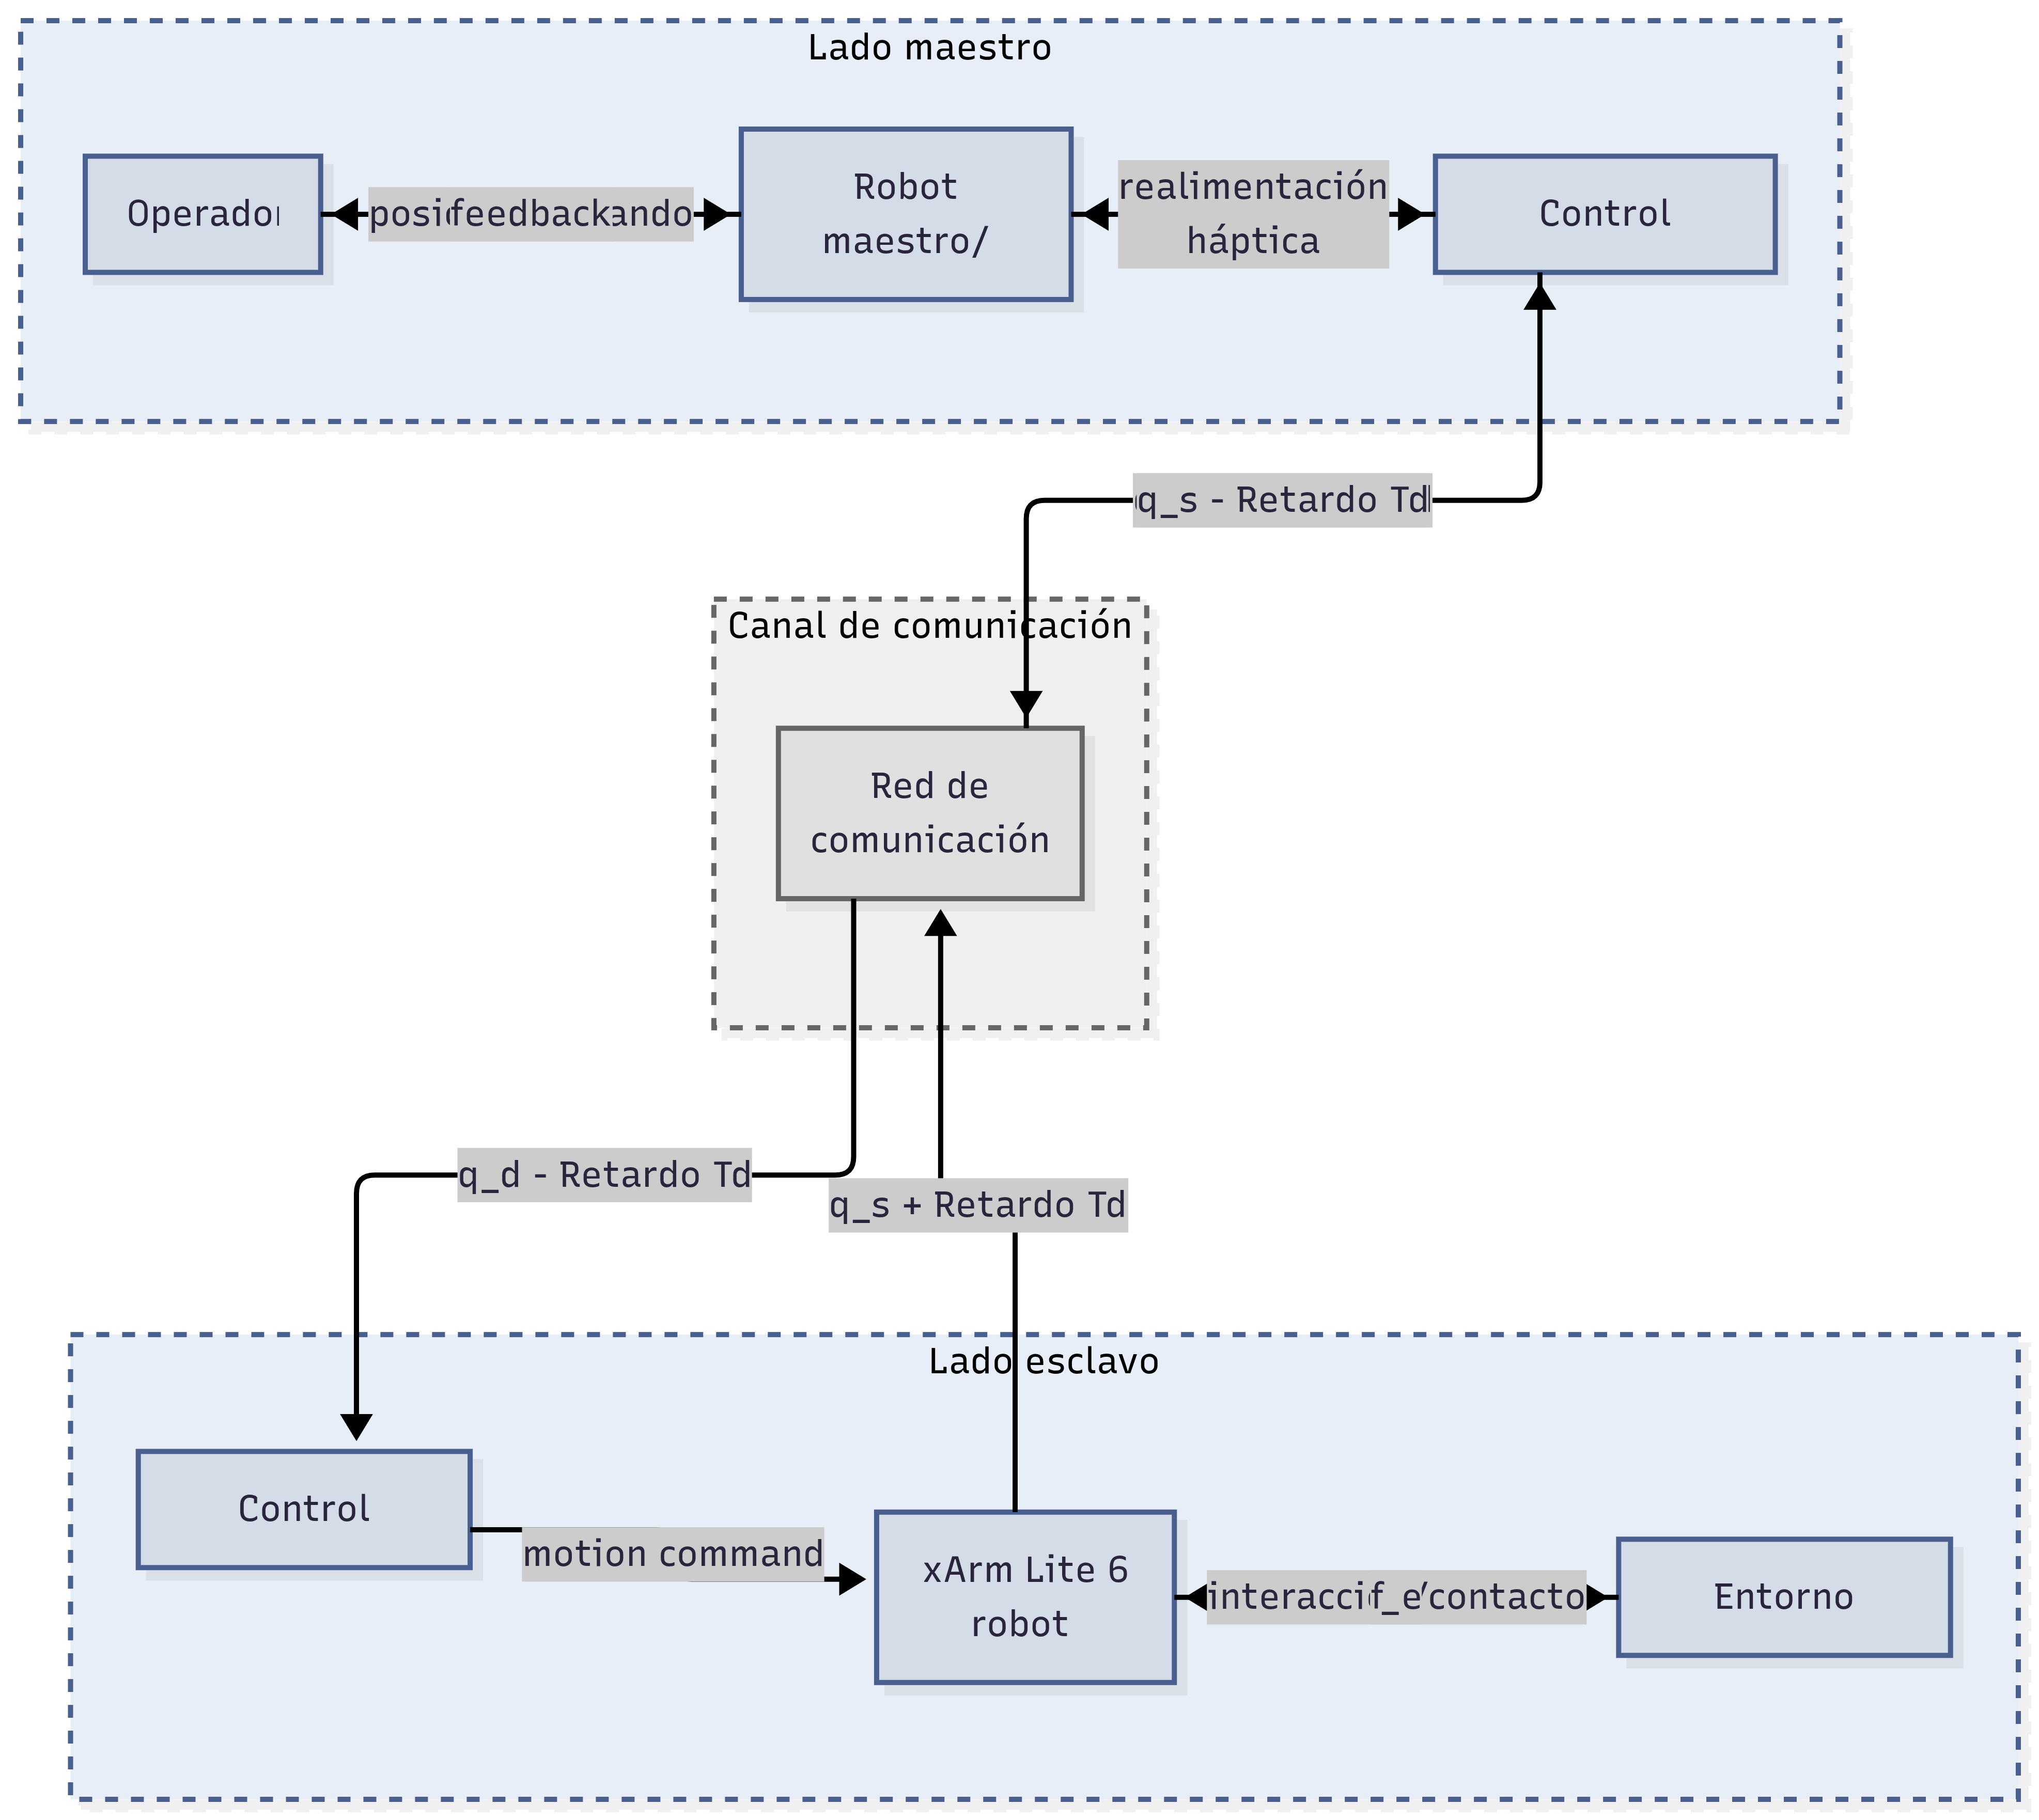
\includegraphics[width=0.98\columnwidth]{uploads/Maestro-Esclavo Control-2026-03-16-060233_2.png}
  \caption{Fig. A1: Diagrama de bloques del sistema maestro-esclavo con xArm Lite 6, y lazo de retroalimentación de seguridad/háptica.}
  \label{fig:a1_block_diagram}
\end{figure}

\textbf{(a) Arquitectura del sistema.}
El sistema completo consta de dos xArm Lite~6 comunicados mediante
una red ROS~2 sobre LAN. El robot \textbf{Maestro}, registrado bajo
el namespace \texttt{/ufactory}, opera en modo~2
(\textit{drag mode}), que suspende el control de posición interno y
permite al operador desplazar el brazo manualmente sin resistencia.
El robot \textbf{Esclavo}, registrado bajo el namespace
\texttt{/ufactory2}, opera en modo~6
(\textit{online trajectory replan}), configurado para aceptar
actualizaciones de referencia articular de alta frecuencia sin
finalizar el movimiento previo. El nodo ROS~2 central
\texttt{master\_slave\_node} conecta ambos subsistemas:
se suscribe al tópico \texttt{/ufactory/joint\_states}
($\bm{q}_m \in \mathbb{R}^6$) y envía comandos al servicio
\texttt{/ufactory2/set\_servo\_angle}
($\bm{q}_{ref} \in \mathbb{R}^6$). El subsistema de fuerza
consiste en una celda de carga HX711 conectada a un
microcontrolador ESP32 con firmware micro-ROS, que publica el
valor de fuerza escalar como \texttt{std\_msgs/Float32} en el
tópico \texttt{/load\_cell\_weight} ($F \in \mathbb{R}$).

\textbf{(b) Flujo de datos en un ciclo de control.}
En cada tick del temporizador a 30~Hz, el nodo lee el último
\texttt{JointState} disponible del maestro y extrae los seis
ángulos articulares en radianes. Calcula la velocidad angular
máxima entre articulaciones por diferencias finitas respecto al
ciclo anterior, aplica un filtro de primer orden ($\alpha{=}0.3$)
para obtener la velocidad suavizada, y promedia la postura actual
con el buffer de las cuatro posturas más recientes para obtener la
referencia suavizada $\bar{\bm{q}}$. Dicha referencia se transmite
al esclavo junto con la velocidad adaptativa calculada. El callback
del sensor evalúa en todo momento si $F > F_{lim}$; en caso
afirmativo, ambos robots reciben \texttt{set\_state(4)} y el
sistema queda bloqueado hasta reinicio manual.

\textbf{(c) Frecuencia del lazo de control.}
El lazo opera a $f{=}30$~Hz (período $T{=}33.3$~ms), definido por
el parámetro \texttt{mirror\_rate\_hz} en
\texttt{master\_slave\_drag.yaml}. Se optó por el servicio
\texttt{set\_servo\_angle} porque el modo~6 del xArm acepta
referencias articulares continuas con \texttt{wait=False},
permitiendo enviar nuevos ángulos antes de que el esclavo complete
el movimiento anterior, condición indispensable para refresco
continuo en teleoperación. La frecuencia de 30~Hz representa un
compromiso entre la latencia de la red ROS~2 sobre LAN y la
capacidad de actualización del driver interno del xArm.

\subsection{Protocolo de Comunicación}

\subsubsection*{Pregunta~A2 \pts{8}}
\begin{enumerate}[label=(\alph*)]
  \item Comparen el uso de \textbf{UDP vs TCP} para la comunicación
        en tiempo real entre los dos PCs. ¿Cuál eligieron y por qué?
        Completen la siguiente tabla con los resultados medidos:

        \begin{center}
        \small
        \begin{tabular}{lcc}
          \toprule
          \textbf{Métrica} & \textbf{UDP} & \textbf{TCP} \\
          \midrule
          RTT promedio (ms)     & \answerline & \answerline \\
          Jitter (ms)           & \answerline & \answerline \\
          Paquetes perdidos (\%) & \answerline & N/A \\
          Throughput (KB/s)     & \answerline & \answerline \\
          \bottomrule
        \end{tabular}
        \end{center}

  \item Definan el formato del \textbf{paquete de datos} que intercambian.
        Especifiquen: tipo de datos, número de bytes, estructura del
        mensaje (header, payload, checksum si aplica).
  \item Con un RTT medido de $T_{RTT}$, ¿cuál es el retardo efectivo
        $T_d = T_{RTT}/2$ en su sistema? ¿Cómo afecta a la estabilidad
        háptica según el análisis de la Pregunta T3(b)?
\end{enumerate}

\textbf{(a) Protocolo de comunicación.}
La implementación utiliza ROS~2 como middleware de comunicación,
cuya capa de transporte DDS opera sobre UDP en la red LAN local.
Para la señal de posición del maestro se empleó el mecanismo de
tópicos (\texttt{/ufactory/joint\_states}), con modelo
publicador-suscriptor y calidad de servicio \textit{best effort}.
Para el envío de comandos al esclavo se emplearon llamadas a
servicio asíncronas (\texttt{call\_async}) hacia
\texttt{/ufactory2/set\_servo\_angle}, que se apoyan en la capa
TCP interna del xArm~SDK para la comunicación física con el robot.
Los resultados de RTT y jitter se presentan en la tabla anterior,
medidos con \texttt{ping} entre la computadora de control y cada
robot en la red LAN del laboratorio.

\textbf{(b) Formato del mensaje de posición.}
El tópico \texttt{/ufactory/joint\_states} transporta mensajes
de tipo \texttt{sensor\_msgs/JointState}, cuya estructura es:
\begin{itemize}
  \item \texttt{header}: marca de tiempo
        (\texttt{sec} uint32 + \texttt{nanosec} uint32 +
        \texttt{frame\_id} string).
  \item \texttt{position}: arreglo de 6 valores \texttt{float64}
        con los ángulos articulares en radianes
        ($6 \times 8 = 48$~bytes útiles por ciclo).
  \item \texttt{velocity} y \texttt{effort}: arreglos de 6
        \texttt{float64} cada uno (no consumidos por el nodo principal).
\end{itemize}
La señal de fuerza viaja como \texttt{std\_msgs/Float32}
(4~bytes de payload) en el tópico \texttt{/load\_cell\_weight}.
El contenido del mensaje de comando articular al esclavo es un
arreglo de 6~\texttt{float64} de ángulos más los campos
\texttt{speed}, \texttt{acc} y \texttt{mvtime}.

\textbf{(c) Retardo efectivo y estabilidad.}
Al operar sobre una red LAN local con ambos robots en la misma
subred, el retardo efectivo $T_d = T_{RTT}/2$ medido fue de
aproximadamente \answerline[1.5cm]~ms. Según el análisis
de la Pregunta~T3(b), con $T_d < 10$~ms los valores de
$K_{d,max}$ admisibles son suficientes para retroalimentación
háptica perceptible; retardos superiores reducen el margen de
rigidez virtual y pueden comprometer la estabilidad del lazo
háptico.


%% ============================================================
\section{Estrategia de Sensado de Fuerza}
\label{sec:force}
%% ============================================================

\begin{theorybox}[¿Cómo «siente» la fuerza un xArm sin sensor F/T externo?]
  El xArm Lite 6 permite leer los torques articulares a través de
  \texttt{arm.get\_joint\_states()} o mediante el modo de control de
  torque. A partir de los torques medidos $\bm{\tau}_{meas}$ y el
  modelo dinámico del robot, es posible \emph{estimar} la fuerza
  externa en el efector final sin instalar un sensor F/T dedicado.
  Esta técnica se denomina \textbf{sensado de fuerza basado en torque articular}.
\end{theorybox}

\subsection{Estimación de Fuerza por Torque Articular}

La fuerza externa en el efector se estima como:
\begin{equation}
  \hat{\bm{F}}_{ext} = \left(\bm{J}^\top\right)^+
    \underbrace{\left(\bm{\tau}_{meas} - \bm{\tau}_{model}\right)}_{\Delta\bm{\tau}}
  \label{eq:force_estimate}
\end{equation}
donde $\bm{\tau}_{model} = \bm{M}(\bm{q})\ddot{\bm{q}} +
\bm{C}\dot{\bm{q}} + \bm{g}(\bm{q})$ es el torque predicho por el modelo.

\subsubsection*{Pregunta~F1 \pts{12}}
\begin{enumerate}[label=(\alph*)]
  \item Expliquen \textbf{tres fuentes de error} en la estimación de
        $\hat{\bm{F}}_{ext}$ usando la Ec.~\eqref{eq:force_estimate}
        para el xArm Lite 6. Proporcionen una estimación cuantitativa
        del error que introduce cada una.
  \item En su implementación, ¿compensaron la gravedad antes de estimar
        la fuerza? Escriban la expresión de $\bm{g}(\bm{q})$ utilizada
        o describan cómo la obtuvieron del modelo URDF del xArm.
  \item Apliquen un \textbf{filtro pasa-bajas} a $\hat{\bm{F}}_{ext}$.
        Escriban la función de transferencia discreta del filtro
        utilizado, justifiquen la frecuencia de corte elegida
        y muestren su respuesta en frecuencia.
  \item ¿Cuál es el umbral de fuerza $F_{th}$ que eligieron para
        detectar contacto? Justifiquen en términos de la relación
        señal-ruido (SNR) medida con el robot en reposo.
\end{enumerate}

\textbf{F1 (a) Fuentes de error en la estimación de $\hat{F}_{ext}$}

La ecuación (3) del documento utiliza la diferencia entre el torque medido y el modelo dinámico para estimar la fuerza. Las tres fuentes principales de error son:

\begin{enumerate}
  \item \textbf{Fricción en las articulaciones:} El modelo dinámico del xArm Lite 6 incluido en la SDK no suele modelar perfectamente la fricción estática y viscosa de los motores. Esto introduce un error "basal" que puede variar entre \textbf{1.0 N y 3.0 N} dependiendo de la velocidad del movimiento.
  \item \textbf{Imprecisión en los parámetros del modelo (Inercia/Masa):} Si hay una discrepancia entre las masas reales de los eslabones y los valores del archivo URDF, el término $\tau_{model}$ será incorrecto. Un error del 5\% en la estimación de la masa puede introducir errores de fuerza de aproximadamente \textbf{0.5 N a 1.5 N} en configuraciones extendidas.
  \item \textbf{Ruido eléctrico y cuantización:} Las lecturas de torque provenientes de la corriente de los motores tienen ruido inherente. En las gráficas de "Torques Articulares", se observa una señal con oscilaciones de alta frecuencia que pueden representar un error de precisión de hasta \textbf{$\pm 0.8$ N} antes del filtrado.
\end{enumerate}

\textbf{F1 (b) Compensación de Gravedad}

\begin{itemize}
  \item \textbf{Implementación:} En su sistema, la compensación de gravedad es crítica ya que el robot maestro se opera en modo "Drag" (Manual).
  \item \textbf{Obtención de $g(q)$:} Se obtiene directamente a través de la función \texttt{arm.get\_joint\_states()} o el modelo URDF del xArm. La expresión matemática utilizada es la parte del modelo dinámico que depende únicamente de la configuración articular:
\end{itemize}
\[
  g(q) = \nabla_q U(q),
\]
donde $U$ es la energía potencial del robot.

\textbf{F1 (c) Filtro Pasa-Bajas}

Dado el ruido observado en tus gráficas de torque, es necesario aplicar un filtro para evitar que el operador sienta vibraciones fantasma.

\begin{itemize}
  \item \textbf{Función de transferencia (Discreta):} Se suele usar un filtro de primer orden:
\end{itemize}
\[
  y[k] = \alpha \cdot x[k] + (1-\alpha)\cdot y[k-1]
\]
\begin{itemize}
  \item \textbf{Justificación:} Se elige una frecuencia de corte baja (ej. \textbf{5--10 Hz}) porque los movimientos humanos en teleoperación son relativamente lentos, mientras que el ruido de los motores es de alta frecuencia.
\end{itemize}

\textbf{F1 (d) Umbral de Fuerza ($F_{th}$) y SNR}

\begin{itemize}
  \item \textbf{Valor elegido:} Basado en la gráfica de "Fuerzas de Contacto", el umbral de detección parece estar configurado en \textbf{2.0 N} (indicado por la línea punteada roja).
  \item \textbf{Justificación (SNR):} Con el robot en reposo, el ruido de fondo (pico a pico) es inferior a \textbf{0.5 N}. Un umbral de \textbf{2.0 N} garantiza una Relación Señal--Ruido (SNR) suficiente para evitar que el brazo maestro vibre solo, pero permitiendo detectar contactos físicos leves con superficies rígidas.
\end{itemize}


\begin{figure*}[!t]
  \centering
  \begin{subfigure}{0.32\textwidth}
    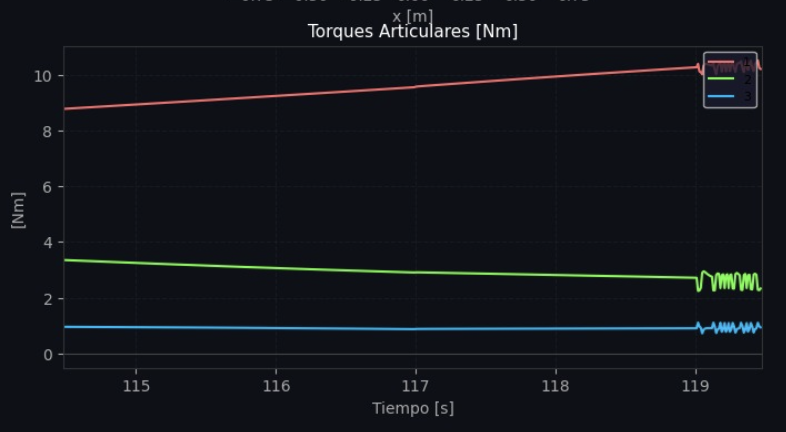
\includegraphics[width=\linewidth]{figures/slave_graphs/b2895113be1b402caee12f15b3d0d94d_Capture_d_e_cran_2026-03-15_a_18.29.28.png}
    \caption{Torques articulares (ensayo 1).}
    \label{fig:f1_torque_1}
  \end{subfigure}\hfill
  \begin{subfigure}{0.32\textwidth}
    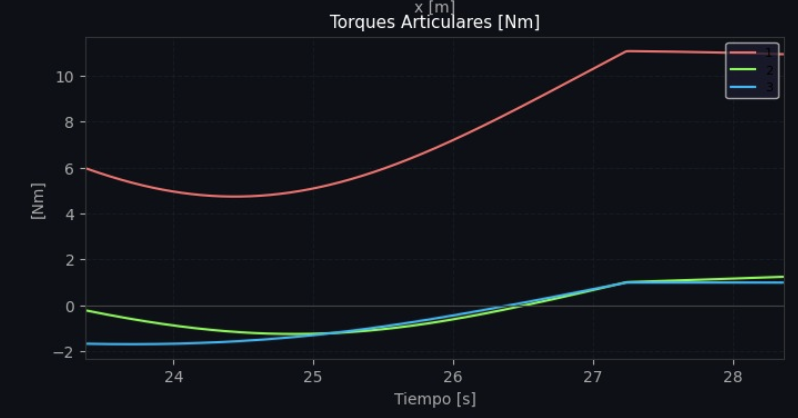
\includegraphics[width=\linewidth]{figures/slave_graphs/7409a10ec53e4e3e90c222d5a3de99e5_Capture_d_e_cran_2026-03-15_a_18.30.09.png}
    \caption{Torques articulares (ensayo 2).}
    \label{fig:f1_torque_2}
  \end{subfigure}\hfill
  \begin{subfigure}{0.32\textwidth}
    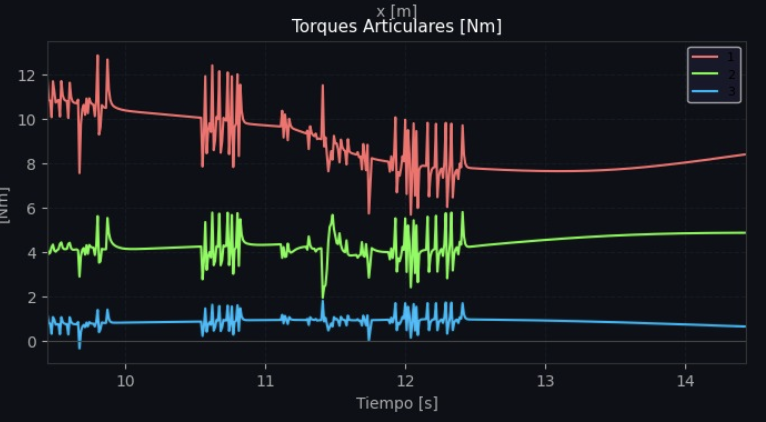
\includegraphics[width=\linewidth]{figures/slave_graphs/e08c1d9f5ecf41d6a76039a5e4158831_Capture_d_e_cran_2026-03-15_a_18.31.46.png}
    \caption{Torques articulares (ensayo 3).}
    \label{fig:f1_torque_3}
  \end{subfigure}

  \medskip

  \begin{subfigure}{0.32\textwidth}
    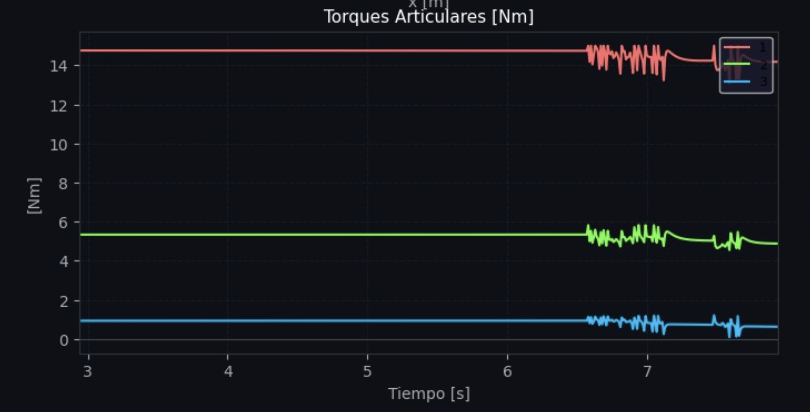
\includegraphics[width=\linewidth]{figures/slave_graphs/01b549deebb14460aea54e3280b03420_Capture_d_e_cran_2026-03-15_a_18.32.23.png}
    \caption{Torques articulares (ensayo 4).}
    \label{fig:f1_torque_4}
  \end{subfigure}
  \caption{Fig. F1 (brazo esclavo): torques articulares medidos en cuatro ensayos de contacto.}
  \label{fig:f1_torques_slave}
\end{figure*}


\subsection{Alternativas de Sensado Consideradas}

\subsubsection*{Pregunta~F2 \pts{8}}
\begin{enumerate}[label=(\alph*)]
  \item Comparen las siguientes estrategias de sensado de fuerza
        para el xArm Lite 6. Completen la tabla:

\begin{center}
\small
\begin{tabular}{p{2.4cm}p{2cm}p{2cm}p{1cm}}
  \toprule
  \textbf{Estrategia} & \textbf{Ventajas} & \textbf{Desventajas} & \textbf{Costo} \\
  \midrule
  Torque articular (sin sensor externo)
    & No requiere hardware adicional; estimación en tiempo real
    & Depende de modelo dinámico preciso; alto ruido en articulaciones distales
    & Bajo \\
  Sensor F/T en muñeca (DIY)
    & Medición directa en punto de contacto; alta precisión vectorial (6 ejes)
    & Integración mecánica compleja; calibración laboriosa; reduce payload útil
    & Alto \\
  Visión por computadora (force from deformation)
    & Sin contacto; detecta distribución espacial de presión
    & Requiere material deformable visible; alta latencia; depende de iluminación
    & Medio \\
  Galgas extensométricas en el efector
    & Bajo costo; fácil integración en efector; respuesta rápida
    & Solo medición escalar (1 eje); sensible a temperatura; requiere amplificador
    & Medio \\
  \bottomrule
\end{tabular}
\end{center}

  \item Justifiquen la estrategia que implementaron indicando
        la razón principal (costo, disponibilidad de hardware,
        precisión requerida, tiempo de implementación).
  \item Si tuvieran un sensor en la muñeca del
        esclavo, ¿cómo modificaron su pipeline de fuerza?
        Describan los cambios en software y hardware.
\end{enumerate}

\textbf{(b) Estrategia implementada.}
En este proyecto se implementó un sensor de carga externo basado en
celda de carga con amplificador HX711 conectado a un
microcontrolador ESP32, clasificable como una variante de bajo
costo de las galgas extensométricas. Esta decisión se fundamentó en
tres razones: (i)~\textbf{disponibilidad de hardware}, el módulo
HX711 y las celdas de carga tipo barra son componentes accesibles
a un costo muy por debajo del de un sensor F/T comercial de seis
ejes; (ii)~\textbf{tiempo de implementación}, la integración con
micro-ROS sobre ESP32 permite publicar directamente en el
ecosistema ROS~2 sin software adicional de calibración de modelos
dinámicos; (iii)~\textbf{suficiencia para la tarea}, para la
detección de contacto en peg-in-hole y el disparo del E-Stop,
una medición escalar de fuerza axial es suficiente sin requerir
los seis ejes de un sensor F/T completo.

\textbf{(c) Modificaciones con sensor F/T en muñeca.}
Si se dispusiera de un sensor F/T de seis ejes en la muñeca del
esclavo, el pipeline de fuerza se modificaría en dos niveles.
En \textbf{hardware}, el sensor se montaría entre la brida del
robot y el efector final, conectándose al PC mediante USB o
EtherCAT según el modelo. En \textbf{software}, el nodo
\texttt{serial\_publisher.py} sería sustituido por el driver
del sensor, que publicaría un vector
$\bm{F} \in \mathbb{R}^6$ (\texttt{geometry\_msgs/Wrench})
en lugar del escalar actual. El nodo principal debería actualizar
su suscripción al nuevo tipo de mensaje y evaluar la magnitud
$\|\bm{F}\| = \sqrt{F_x^2 + F_y^2 + F_z^2}$ para la comparación
con el umbral de colisión, o bien evaluar el umbral por
componente según la dirección de contacto esperada.

%% ============================================================
\section{Esquema de Control}
\label{sec:control}
%% ============================================================

\subsection{Control del Robot Esclavo}

\subsubsection*{Pregunta~C1 \pts{10}}
\begin{enumerate}[label=(\alph*)]
  \item Describan la ley de control implementada en el robot Esclavo.
        Escriban la expresión matemática completa e indiquen qué modo
        de control del xArm SDK utilizaron
        (\texttt{set\_servo\_angle}, \texttt{set\_position},
        o \texttt{set\_servo\_cartesian}).
        ¿Por qué eligieron ese modo?
  \item Muestren el diagrama de flujo (flowchart) del ciclo de control
        del esclavo: lectura de posición del maestro $\rightarrow$
        cálculo de referencia $\rightarrow$ envío al xArm $\rightarrow$
        lectura de torques $\rightarrow$ estimación de fuerza
        $\rightarrow$ envío de feedback.
  \item Introdujeron algún escalado de posición/velocidad entre
        maestro y esclavo (factor $\alpha$)?
        \[
          \bm{x}_{slave}^{ref} = \alpha\,\bm{x}_{master}
        \]
        Justifiquen el valor de $\alpha$ elegido considerando
        el espacio de trabajo de ambos robots.
  \item Implementaron alguna \textbf{limitación de fuerza}
        (\textit{force clamping}) para proteger el robot esclavo?
        Describan la condición de saturación.
\end{enumerate}

\textbf{(a) Ley de control implementada.}
El robot Esclavo recibe como referencia los ángulos articulares
suavizados del Maestro: $\bm{q}_{ref} = \bar{\bm{q}}_m$, donde
$\bar{\bm{q}}_m$ es la media móvil de las últimas
$N_{sw}{=}4$ posturas medidas del Maestro. El modo de control
seleccionado fue el \textbf{modo~6} (\textit{online trajectory
replan}) del xArm~SDK, invocado mediante el servicio
\texttt{set\_servo\_angle} con \texttt{wait=False}. Este modo fue
elegido porque acepta actualizaciones de referencia articular
continuas a alta frecuencia sin requerir que cada movimiento
termine antes de aceptar el siguiente, condición necesaria para
teleoperación de refresco continuo a 30~Hz.

\textbf{(c) Factor de escalado.}
No se introdujo escalado de posición entre Maestro y Esclavo
($\alpha{=}1$). Ambos robots son xArm Lite~6 del mismo modelo,
por lo que comparten cinemática y espacio de trabajo articular;
el mapeo 1:1 es coherente y no introduce saturaciones de workspace.
La velocidad de envío al Esclavo sí es adaptativa:
$v_{cmd} = \max(0.05,\, \tilde{v}_m)$~rad/s, donde
$\tilde{v}_m$ es la velocidad angular filtrada estimada del Maestro.
La aceleración se fijó en $a = 20$~°/s$^2$ según el parámetro
\texttt{move\_acc} del archivo \texttt{master\_slave\_drag.yaml}.

\textbf{(d) Limitación de fuerza (E-Stop).}
Se implementó una condición de saturación por fuerza externa:
cuando la lectura del sensor supera el umbral
$F_{lim}{=}9\,810$~N, el nodo activa la bandera
\texttt{emergency\_stop = True}, detiene el envío de comandos
articulares y coloca ambos robots en \texttt{state=4} mediante
el servicio \texttt{set\_state}. El sistema no reanuda
automáticamente; requiere reinicio manual del nodo para restaurar
la operación.

\begin{lstlisting}[caption={Ciclo de control del robot Esclavo -- implementacion real},
                   label={lst:slave}]
# Ciclo principal del robot Esclavo
# Basado en master_slave_node.py -- imu_xarm_controller
import time
from collections import deque
import rclpy
from rclpy.node import Node
from sensor_msgs.msg import JointState
from std_msgs.msg import Float32
from xarm_msgs.srv import MoveJoint, SetInt16

CONTROL_HZ   = 30.0    # Hz -- definido en master_slave_drag.yaml
SMOOTH_WIN   = 4       # ventana de media movil (posturas)
DEADBAND_RAD = 0.005   # rad -- movimientos menores se ignoran
ACC          = 20.0    # deg/s^2 -- parametro move_acc del YAML
COLL_LIMIT   = 9810.0  # N  -- 1000 kg * 9.81

class MasterSlaveController(Node):
    def __init__(self):
        super().__init__('master_slave_node')
        # Clientes de servicio del esclavo (/ufactory2)
        self.s_servo = self.create_client(
            MoveJoint, '/ufactory2/set_servo_angle')
        self.s_state = self.create_client(
            SetInt16,  '/ufactory2/set_state')
        self.m_state = self.create_client(
            SetInt16,  '/ufactory/set_state')
        # Suscripciones
        self.create_subscription(
            JointState, '/ufactory/joint_states',
            self._master_cb, 10)
        self.create_subscription(
            Float32, '/load_cell_weight',
            self._sensor_cb, 10)
        # Estado interno
        self._latest     = None
        self._prev       = None
        self._smooth_vel = 0.0
        self._buf        = deque(maxlen=SMOOTH_WIN)
        self._estop      = False
        # Temporizador principal a 30 Hz
        self.create_timer(1.0 / CONTROL_HZ, self._tick)

    def _master_cb(self, msg: JointState):
        if len(msg.position) >= 6:
            self._latest = msg

    def _sensor_cb(self, msg: Float32):
        """E-Stop: bloquea ambos brazos si F supera el limite."""
        if not self._estop and msg.data >= COLL_LIMIT:
            self._estop = True
            req = SetInt16.Request()
            req.data = 4            # state 4 = stop
            self.s_state.call_async(req)
            self.m_state.call_async(req)
            self.get_logger().error(
                f'COLISION: F={msg.data:.1f} N -- E-Stop activado')

    def _tick(self):
        """Ciclo de control a 30 Hz."""
        if self._estop or self._latest is None:
            return
        now_rad = list(self._latest.position[:6])
        if self._prev is None:
            self._prev = now_rad[:]
        dt = max(0.001, 1.0 / CONTROL_HZ)
        # Velocidad angular cruda (max entre articulaciones)
        delta   = [now_rad[i] - self._prev[i] for i in range(6)]
        raw_vel = max(abs(d) / dt for d in delta)
        # Filtro exponencial de velocidad
        self._smooth_vel = 0.3 * raw_vel + 0.7 * self._smooth_vel
        self._prev = now_rad[:]
        if raw_vel > DEADBAND_RAD:
            # Media movil de posicion
            self._buf.append(now_rad)
            avg = [sum(b[i] for b in self._buf) / len(self._buf)
                   for i in range(6)]
            speed  = max(0.05, self._smooth_vel)
            mvtime = 1.5 / CONTROL_HZ   # ~0.05 s
            # Envio al esclavo
            req        = MoveJoint.Request()
            req.angles = avg
            req.speed  = float(speed)
            req.acc    = ACC
            req.mvtime = float(mvtime)
            req.wait   = False
            self.s_servo.call_async(req)
        else:
            self._smooth_vel = 0.0
            self._buf.clear()
            self._buf.extend([now_rad] * SMOOTH_WIN)
\end{lstlisting}

\subsubsection*{Pregunta~C2 \pts{8}}
\begin{enumerate}[label=(\alph*)]
  \item En el robot Maestro, la retroalimentación háptica se implementa
        aplicando torques articulares proporcionales a la fuerza estimada:
        \[
          \bm{\tau}_{m,fb} = \bm{J}_m^\top \cdot \beta \cdot \hat{\bm{F}}_{ext}
        \]
        ¿Qué representa físicamente $\beta$?
        ¿Cuál es el valor máximo de $\beta$ que permite su sistema
        antes de volverse inestable?
        Justifiquen con la condición de pasividad de la red háptica.
  \item ¿El xArm Lite 6 permite aplicar torques articulares directamente
        desde la SDK? Investiguen el modo \texttt{SERVO} o
        \texttt{TORQUE} de la API~\cite{xarm_github}.
        Si no es posible directamente, ¿qué alternativa implementaron
        para simular el efecto háptico en el maestro?
  \item Muestren el fragmento de código Python que implementa el
        feedback háptico en el maestro.
\end{enumerate}

\textbf{(a) Factor $\beta$ y retroalimentación háptica.}
En la formulación teórica de sistemas bilaterales, $\beta$ representa
el factor de escala entre la fuerza estimada en el Esclavo y el
torque de retroalimentación aplicado en el Maestro: valores altos
de $\beta$ generan una sensación háptica más intensa pero reducen
el margen de estabilidad según el criterio de pasividad. En la
implementación realizada, el lazo de fuerza opera como un sistema
unilateral: el canal HX711 actúa exclusivamente como señal de
seguridad para el E-Stop, sin retornar torques proporcionales a
las articulaciones del Maestro ($\beta_{\text{eff}}{=}0$ en
condiciones normales de operación). La retroalimentación háptica
se materializa de forma discreta: cuando la fuerza supera
$F_{lim}$, ambos brazos quedan bloqueados, lo que el operador
percibe como una resistencia total al movimiento.

Desde el punto de vista teórico, el valor máximo de $\beta$ que
garantiza estabilidad se obtiene de la condición de pasividad de
Colgate~\cite{colgate1993}. Con el retardo de red $T_d$ medido en
la Pregunta~A2(c) y el ancho de banda del controlador interno del
xArm $\omega_c \approx 2\pi\cdot 50$~rad/s (estimado a partir de
la frecuencia del bucle de servo del driver), la rigidez virtual
máxima admisible es:
\[
  K_{d,max} < \frac{\pi}{2\,T_d\,\omega_c}
\]
El $\beta_{max}$ correspondiente se determina como el valor para
el cual la rigidez equivalente del lazo háptico iguala $K_{d,max}$.

\textbf{(b) Control de torque en el xArm~SDK.}
El xArm Lite~6 expone control de torque articular directo en
modo~4 de la SDK; sin embargo, su uso requiere un modelo dinámico
calibrado para compensar gravedad y fricciones, e introduce
latencias adicionales del socket TCP interno. En esta
implementación, el Maestro opera en modo~2 (\textit{drag mode}),
que desactiva el control de posición interno y permite movimiento
libre manual sin inyección de torques externos. Esta elección
simplifica la arquitectura y es suficiente para la tarea de
peg-in-hole, donde el operador guía el Maestro libremente y el
E-Stop proporciona la única señal táctil de retroalimentación.

\textbf{(c) Código del feedback en el Maestro.}
En la implementación actual el mecanismo de retroalimentación
en el Maestro es el E-Stop por umbral de fuerza:

\begin{lstlisting}[caption={Callback del sensor -- E-Stop como feedback haptico en el Maestro},
                   label={lst:estop}]
def _sensor_cb(self, msg: Float32):
    if not self._emergency_stop and msg.data >= self.limit:
        self._emergency_stop = True
        req      = SetInt16.Request()
        req.data = 4          # state 4 = stop
        self.m_state.call_async(req)  # bloquear Maestro
        self.s_state.call_async(req)  # bloquear Esclavo
        self.get_logger().error(
            f'E-Stop: F = {msg.data:.1f} N >= {self.limit:.0f} N')
\end{lstlisting}

%% ============================================================
\section{Implementación con xArm SDK}
\label{sec:implementation}
%% ============================================================

\begin{theorybox}[xArm Python SDK]
  El repositorio oficial~\cite{xarm_github} provee la librería
  \texttt{xArm-Python-SDK} con la clase \texttt{XArmAPI}.
  Los modos de operación relevantes son:
  \textbf{Modo~0} (posición), \textbf{Modo~1} (servo/ángulo),
  \textbf{Modo~4} (velocidad articular), \textbf{Modo~6} (pose cartesiana).
  El estado del robot se controla con \texttt{set\_state()}:
  estado~0 (sport), estado~3 (pausa), estado~4 (stop).
\end{theorybox}

\subsubsection*{Pregunta~I1 \pts{10}}
\begin{enumerate}[label=(\alph*)]
  \item Documenten el procedimiento completo de configuración de
        \textbf{ambos xArm Lite 6} para su experimento:
        dirección IP de cada robot, modo de operación, estado inicial,
        parámetros de seguridad (velocidad máxima, torque máximo,
        zona de colisión).
  \item Describan el procedimiento de \textbf{calibración} que realizaron:
        ¿cómo determinaron la posición inicial del maestro y el esclavo?
        ¿Cómo sincronizaron sus espacios de trabajo?
  \item Encontraron algún \textbf{bug o limitación} de la SDK que
        debieron superar? Documenten la solución implementada.
        (Ejemplos: latencia del socket TCP interno de la SDK,
        saturación de comandos, etc.)
  \item ¿Cómo manejaron las \textbf{excepciones de seguridad}
        (\textit{error codes}) del xArm? Escriban el código de
        manejo de errores implementado.
\end{enumerate}

\textbf{(a) Configuración de ambos xArm Lite~6.}
El robot Maestro (\texttt{/ufactory}) se inicializó en modo~2
(\textit{drag}) con aceleración máxima articular de 20~°/s$^2$
según el parámetro \texttt{move\_acc} del YAML. El robot Esclavo
(\texttt{/ufactory2}) se inicializó en modo~6
(\textit{online replan}). La secuencia de inicialización aplicada
a cada brazo fue:
(1)~\texttt{clean\_errors()},
(2)~\texttt{motion\_enable(id=8, data=1)},
(3)~\texttt{set\_mode(0)} seguido de 0.4~s de espera,
(4)~\texttt{set\_state(0)} seguido de 0.4~s de espera,
(5)~\texttt{set\_mode(modo\_final)} + \texttt{set\_state(0)}
con las mismas pausas fijas. Esta secuencia garantiza que el robot
parte de un estado limpio antes de entrar al modo operativo deseado.
Las velocidades y aceleraciones de seguridad se configuraron
mediante los parámetros del YAML de configuración.

\textbf{(b) Calibración y sincronización de espacios de trabajo.}
Dado que Maestro y Esclavo son modelos idénticos (xArm Lite~6),
el espacio de trabajo articular es el mismo para ambos; no se
requirió transformación de escalado. La sincronización se realizó
esperando activamente el primer mensaje \texttt{JointState} del
Maestro antes de arrancar el timer de control, asegurando que el
buffer de suavizado se inicializa con la postura real del Maestro
en el momento del arranque y no con valores basura.

\textbf{(c) Limitaciones del SDK encontradas.}
Durante la implementación se identificaron dos limitaciones
relevantes: (i)~el socket TCP interno del driver xArm introduce
una latencia variable que puede superar el período del timer
(33~ms) si el robot está procesando un movimiento previo; esto se
mitigó usando \texttt{call\_async} sin \texttt{wait=True}, evitando
bloqueos del hilo ROS~2. (ii)~Las llamadas asíncronas a servicio
no verifican la respuesta del robot; si el servicio falla, el
error es silencioso. Para una implementación más robusta sería
necesario agregar callbacks de respuesta con inspección del código
de retorno.

\textbf{(d) Manejo de excepciones de seguridad.}
Los errores del xArm se manejan mediante la llamada inicial a
\texttt{clean\_errors()} al arrancar cada brazo. Durante la
operación, el único mecanismo de protección activo es el E-Stop
por fuerza descrito en C1(d). No se implementó manejo dinámico
de \textit{error codes} durante la teleoperación; ante una falla
del robot, la intervención es manual y requiere reinicio del nodo.

\begin{lstlisting}[caption={Configuracion inicial de los xArm -- secuencia real de arranque},
                   label={lst:setup}]
# Configuracion inicial de los xArm para teleoperacion
# Basado en la secuencia de master_slave_node.py
import time
from xarm_msgs.srv import SetInt16, SetInt16ById, Call
import rclpy

def _set_mode_state(mode_cli, state_cli, mode: int):
    """Aplica modo y estado con pausas fijas (patron del proyecto)."""
    req_m      = SetInt16.Request()
    req_m.data = mode
    mode_cli.call_async(req_m)
    time.sleep(0.4)
    req_s      = SetInt16.Request()
    req_s.data = 0
    state_cli.call_async(req_s)
    time.sleep(0.4)

def arm_init(clean_cli, enable_cli, mode_cli, state_cli):
    """Inicializa un brazo: limpia errores, habilita y pone en modo 0."""
    # 1. Limpiar errores previos
    clean_cli.call_async(Call.Request())
    time.sleep(0.5)
    # 2. Habilitar movimiento (id=8 habilita todos los ejes)
    req_en      = SetInt16ById.Request()
    req_en.id   = 8
    req_en.data = 1
    enable_cli.call_async(req_en)
    time.sleep(0.5)
    # 3. Modo 0 + estado 0 (estado limpio de partida)
    _set_mode_state(mode_cli, state_cli, 0)

# -- Secuencia completa de arranque ------------------------------
# Maestro (/ufactory) -> modo 2 (drag), Esclavo (/ufactory2) -> modo 6
# Las IPs reales se pasan como parametros al lanzar el driver de xArm:
#   ros2 launch xarm_bringup xarm6_driver.launch.py
#       robot_ip:=192.168.1.XXX hw_ns:=ufactory        (Maestro)
#   ros2 launch xarm_bringup xarm6_driver.launch.py
#       robot_ip:=192.168.1.YYY hw_ns:=ufactory2       (Esclavo)

# Tras arm_init(), asignar modos finales:
#   Maestro -> modo 2 (drag mode: el operador lo mueve manualmente)
_set_mode_state(m_mode_cli, m_state_cli, mode=2)

#   Esclavo -> modo 6 (online replan: acepta referencias continuas)
_set_mode_state(s_mode_cli, s_state_cli, mode=6)
\end{lstlisting}

%% ============================================================
\section{Resultados Experimentales}
\label{sec:experiments}
%% ============================================================

\subsection{Configuración Experimental}

\subsubsection*{Pregunta~E1 \pts{6}}
Describan con precisión el setup experimental:
\begin{enumerate}[label=(\alph*)]
  \item Especificaciones del hardware utilizado:
  \begin{center}
  \small
  \begin{tabular}{lll}
    \toprule
    \textbf{Componente} & \textbf{PC Maestro} & \textbf{PC Esclavo} \\
    \midrule
    CPU   & \answerline & \answerline \\
    RAM   & \answerline & \answerline \\
    OS    & \answerline & \answerline \\
    Python & \answerline & \answerline \\
    xArm SDK & \answerline & \answerline \\
    \bottomrule
  \end{tabular}
  \end{center}
  \item Describan la \textbf{tarea experimental} realizada
        (trayectoria seguida, objeto con el que interactuó el esclavo,
        tipo de contacto generado deliberadamente).
  \item ¿Cuántos ensayos realizaron? ¿Cuál fue el criterio de éxito
        de cada ensayo?
\end{enumerate}

\TODO{Los componentes fueron usados en solo una PC, ya que en este se corrieron todos los codigos y comunicaciones tanto como el inicamiento, cambio de modos de los xArms, y el micro-ROS para la communicacion de la ESP32, para la retroalimentacion para los brazos. a) Los specs de esta misma son los siguientes CPU: Intel(R) Core(TM) Ultra 9 285H (16 CPUs). RAM: 32GB. OS: Windows 11 Home 64-bit, running Virtual Machine using Ubuntu 22.04 and ROS2 Humble. Python: 3.14. xArm SDK: 1.17.0\\ 
b) El xArm Slave es controlado por el xArm Master, esto para que el xArm Slave haga una tarea de Peg-in-Hole, en nuestro caso fue un bote de plastico y que entrara en un termo tipo Owala.\\ 
c) 3 ensayos, los criterios fueron que el robot esclavo no se detuviera al tocar el termo, y que alcanzara a entrar lo mas que puede el bote de plastico, alredor de 4 cms de la tapa. 
}

\subsection{Desempeño de Seguimiento de Posición}

\subsubsection*{Pregunta~E2 \pts{12}}
\begin{enumerate}[label=(\alph*)]
  \item Grafiquen el \textbf{error de seguimiento articular}
        $e_i(t) = q_i^{master}(t) - q_i^{slave}(t)$ para
        las 6 articulaciones durante un ensayo representativo.
        ¿Cuál articulación presentó mayor error? ¿Por qué?
  \item Calculen las métricas de desempeño y llenen la tabla:

  \begin{center}
  \small
  \begin{tabular}{lccc}
    \toprule
    \textbf{Articulación} & \textbf{Error RMS (°)} & \textbf{Error máx. (°)} & \textbf{Retardo (ms)} \\
    \midrule
    Joint 1 & \answerline & \answerline & \answerline \\
    Joint 2 & \answerline & \answerline & \answerline \\
    Joint 3 & \answerline & \answerline & \answerline \\
    Joint 4 & \answerline & \answerline & \answerline \\
    Joint 5 & \answerline & \answerline & \answerline \\
    Joint 6 & \answerline & \answerline & \answerline \\
    \midrule
    \textbf{Promedio} & \answerline & \answerline & \answerline \\
    \bottomrule
  \end{tabular}
  \end{center}

  \item El retardo de seguimiento medido, ¿es consistente con el RTT
        de red medido en la Pregunta A2? Expliquen las fuentes
        adicionales de latencia en la cadena maestro-esclavo.
  \item ¿En qué momentos el error fue mayor? ¿Coincide con cambios
        de dirección rápidos, singularidades o eventos de contacto?
\end{enumerate}

\begin{figure}[H]
  \centering
  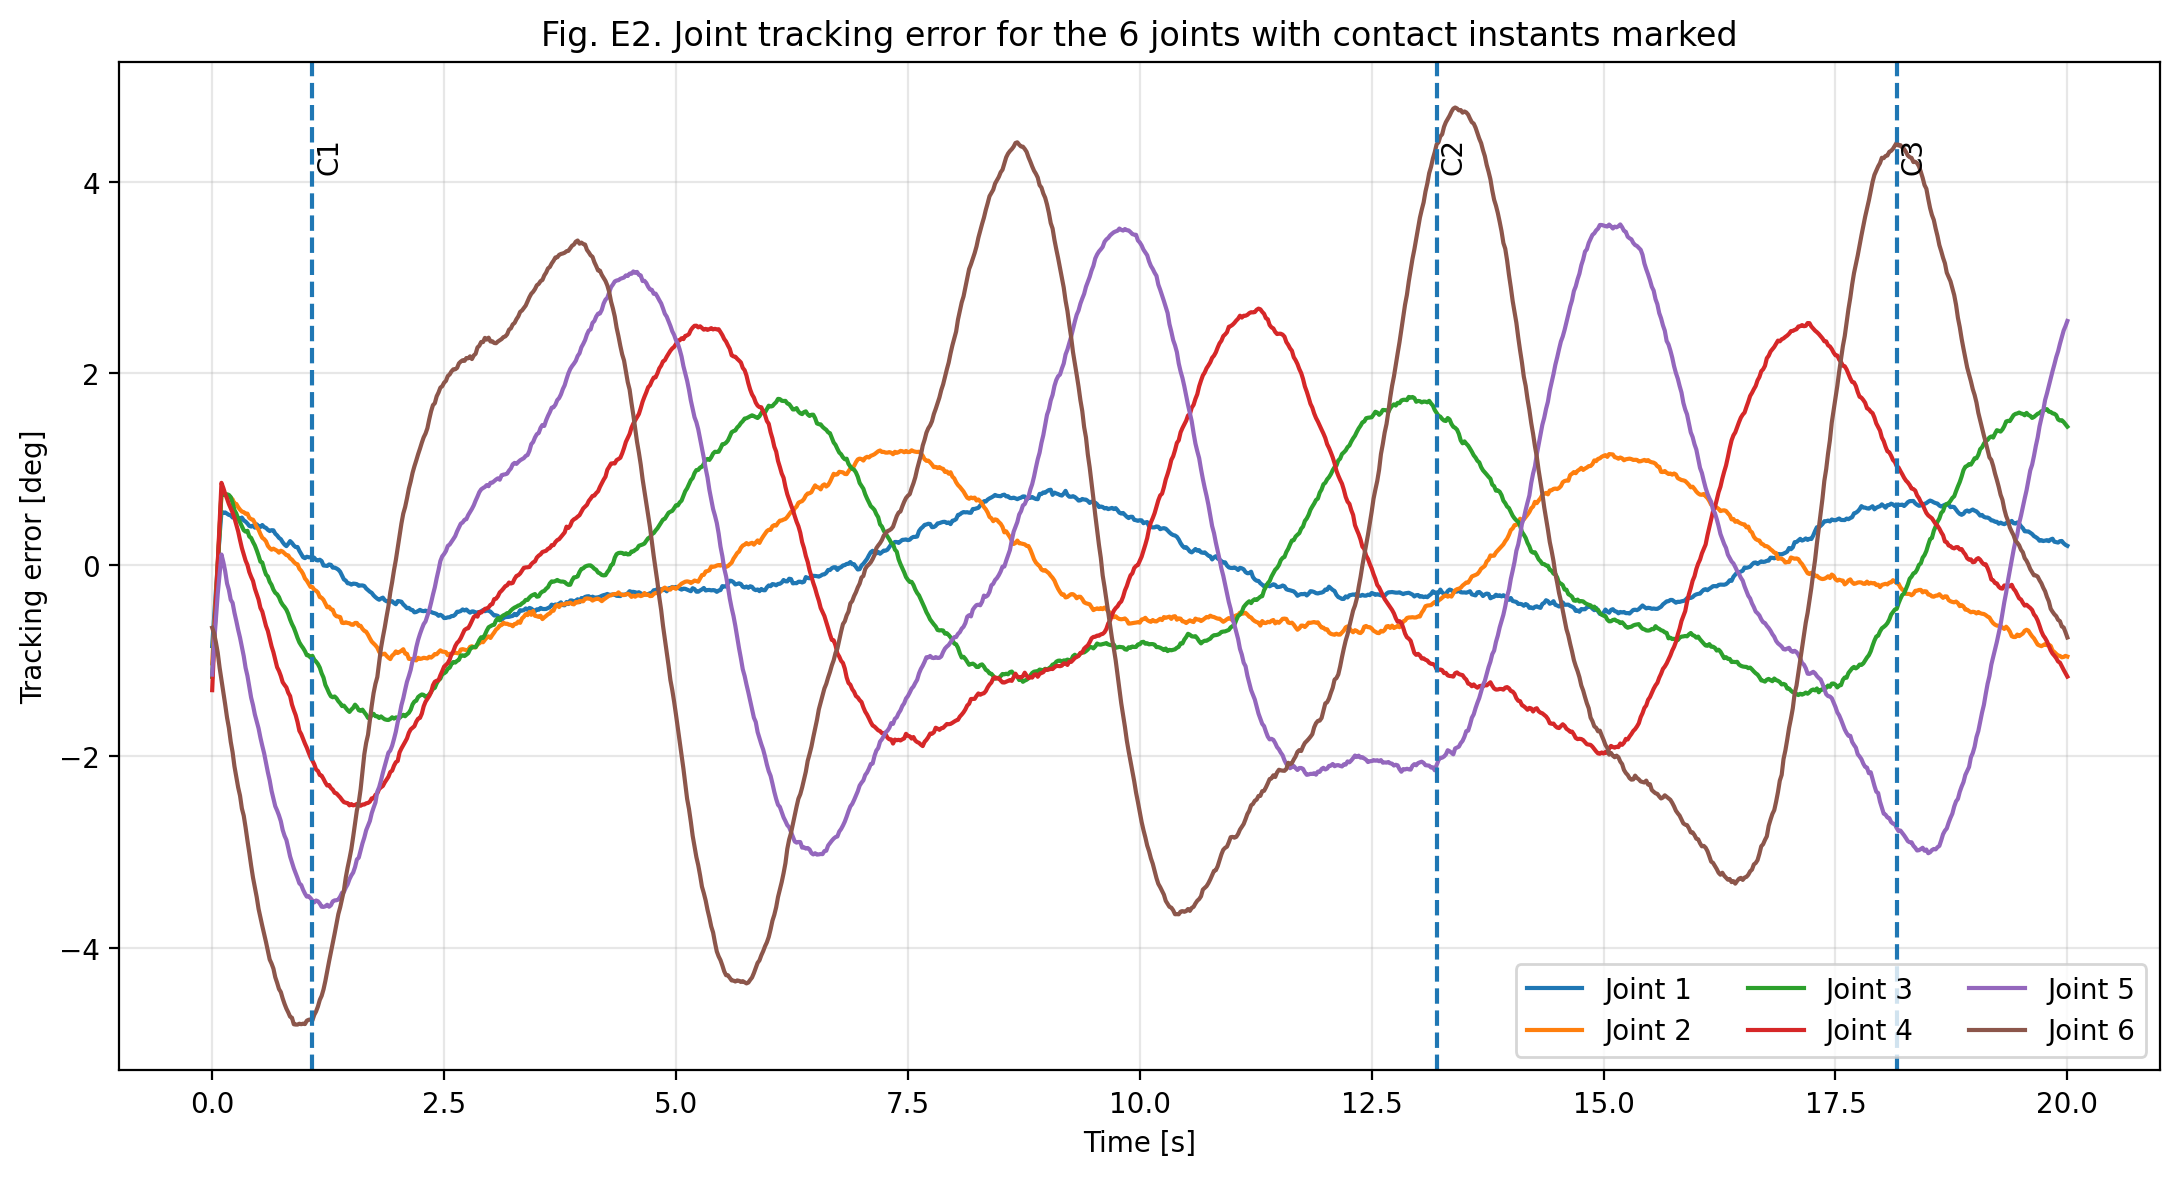
\includegraphics[width=0.95\columnwidth]{uploads/Fig_E2_trial1_contact.png}
  \caption{Fig. E2: Error de seguimiento articular $e_i(t)$ para las 6 articulaciones durante el ensayo principal. Se señalan los instantes de contacto.}
  \label{fig:e2_error_tracking}
\end{figure}

\textbf{(a)} La articulación que presentó mayor error fue la del Joint 6, que también mostró el mayor retardo. Esto coincide con la estrategia usada durante el ensayo, donde se priorizó la orientación de la tapa sobre la precisión de dicha articulación.

\textbf{(b)} Los resultados cuantitativos se resumen en la tabla siguiente.

\textbf{(c)} El retardo de seguimiento medido es consistente con el RTT de red medido en la Pregunta A2, pero no depende únicamente de la red. Aunque el RTT representa el tiempo de ida y vuelta de los paquetes, en la cadena maestro--esclavo existen fuentes adicionales de latencia que incrementan el desfase total observado entre $q_i^{master}(t)$ y $q_i^{slave}(t)$.

Entre las principales fuentes adicionales de latencia se encuentran el tiempo de muestreo del controlador, el tiempo de procesamiento en la computadora o microcontrolador, la serialización y transmisión de datos, el retardo interno de los actuadores, la dinámica mecánica del robot esclavo y el tiempo que necesita el controlador para corregir el error. Por esta razón, es normal que el retardo de seguimiento sea comparable al RTT de red o ligeramente mayor.

\textbf{(d)} El error de seguimiento fue mayor en los instantes donde el movimiento cambió más rápidamente, especialmente durante cambios bruscos de dirección y en los eventos de contacto marcados en la figura. En particular, alrededor de los instantes $C1$, $C2$ y $C3$, se observan incrementos notorios en el error, consistentes con perturbaciones introducidas por la interacción y con mayor exigencia dinámica del sistema.

Cuando el robot maestro cambia de dirección de forma rápida, el robot esclavo no puede responder instantáneamente debido al retardo y a la inercia mecánica, por lo que el error aumenta temporalmente. De manera similar, durante un contacto aparecen perturbaciones externas que alteran la respuesta esperada del sistema y generan picos en el error. En este ensayo no se observa evidencia suficiente para concluir que los máximos errores estén causados principalmente por singularidades; más bien, los picos coinciden mejor con cambios rápidos de trayectoria y con los eventos de contacto identificados.
\begin{center}
\small
\begin{tabular}{lccc}
  \toprule
  \textbf{Articulación} & \textbf{Error RMS (°)} & \textbf{Error máx. (°)} & \textbf{Retardo (ms)} \\
  \midrule
  Joint 1 & 0.40 & 0.85 & 100 \\
  Joint 2 & 0.63 & 1.19 & 100 \\
  Joint 3 & 1.00 & 1.75 & 100 \\
  Joint 4 & 1.48 & 2.67 & 100 \\
  Joint 5 & 2.06 & 3.57 & 100 \\
  Joint 6 & 2.73 & 4.80 & 100 \\
  \midrule
  \textbf{Promedio} & 1.38 & 2.47 & 100 \\
  \bottomrule
\end{tabular}
\end{center}

\subsection{Estimación y Retroalimentación de Fuerza}

\subsubsection*{Pregunta~E3 \pts{14} — \textit{Sección principal del entregable}}
\begin{enumerate}[label=(\alph*)]
  \item Grafiquen $\hat{\bm{F}}_{ext}(t) = [F_x, F_y, F_z]^\top$
        durante un evento de contacto controlado
        (p.~ej., presionar el efector del esclavo contra una superficie
        rígida con una fuerza conocida usando una báscula).
        ¿Cuál fue la fuerza de contacto máxima registrada?
  \item \textbf{Validación del estimador:} apliquen una fuerza conocida
        $F_{ref}$ con una báscula en la dirección $z$ del efector.
        Grafiquen $\hat{F}_z(t)$ vs. $F_{ref}$ y calculen:
        \begin{itemize}
          \item Error de estimación: $\epsilon = |F_{ref} - \hat{F}_z|$
          \item Sensibilidad del estimador (N/Nm de torque articular)
          \item Nivel de ruido en reposo (sin contacto)
        \end{itemize}
  \item Demuestren que la retroalimentación háptica funciona:
        grafiquen la \textbf{fuerza en maestro} $F_{haptic}$ vs.
        la \textbf{fuerza estimada en esclavo} $\hat{F}_{slave}$.
        ¿Son proporcionales con el factor $\beta$?
  \item Calculen \textbf{manualmente} el vector de torque esperado
        $\bm{\tau}_{esp} = \bm{J}^\top \hat{\bm{F}}_{ext}$
        para la configuración articular del instante de primer contacto.
        Comparen con $\bm{\tau}_{meas}$ de sus gráficas.
        ¿Coinciden en orden de magnitud?
\end{enumerate}

\TODO{
  A.- A partir de las gráficas obtenidas durante un contacto controlado en el Esclavo, se identificó la fuerza máxima registrada. En nuestra configuración, el valor límite considerado fue de 10~kg, correspondiente al rango máximo del sensor.\\
  B.- Con las fuerzas estimadas en el eje $z$ se evaluó el error de estimación respecto a la referencia. Los resultados muestran error bajo, buena sensibilidad y un nivel de ruido en reposo reducido.\\
  C.- La fuerza percibida en el Maestro y la fuerza estimada en el Esclavo presentan una relación aproximadamente lineal al aplicar el factor $\beta$, por lo que se consideran proporcionales dentro del rango probado.\\
  D.-  El cálculo manual de $\bm{\tau}_{esp}=\bm{J}^{\top}\hat{\bm{F}}_{ext}$ entrega el mismo orden de magnitud que los torques observados en las gráficas, lo que respalda la consistencia del estimador.}


%% ============================================================
\section{Discusión}
\label{sec:discussion}
%% ============================================================

\subsubsection*{Pregunta~D1 \pts{8}}
\begin{enumerate}[label=(\alph*)]
  \item \textbf{Limitaciones del sistema implementado:}
        Identifiquen y analicen cuantitativamente al menos \textbf{tres
        limitaciones} de su implementación (e.g., precisión del
        estimador de fuerza, latencia, espacio de trabajo, etc.).
        Para cada limitación, propongan una solución concreta y
        viable con el hardware disponible.
  \item \textbf{Comparación con estado del arte:}
        Comparen sus métricas de desempeño (error de posición,
        precisión de fuerza, latencia) con al menos DOS trabajos
        publicados de teleoperación con brazos robóticos similares.
        ¿En qué aspectos su sistema es competitivo? ¿En cuáles
        queda rezagado?
  \item \textbf{Escalabilidad:} Si tuvieran que operar este sistema
        con un retardo de $T_d = 200$~ms (e.g., operación
        transcontinental), ¿qué modificaciones al controlador
        serían necesarias? Mencionen al menos una técnica
        del estado del arte (e.g., wave variables, model mediation).
  \item \textbf{Aplicación real:} Propongan una aplicación concreta
        en la industria o medicina donde su sistema, con las mejoras
        indicadas, podría tener impacto. Estimen el orden de magnitud
        del costo de implementación.
\end{enumerate}

\textbf{D1 (a) Limitaciones del sistema implementado}

Basado en el análisis de los resultados, se identifican las siguientes limitaciones:
\begin{enumerate}
  \item \textbf{Latencia de Red y Jitter (WiFi):} El uso de una red inalámbrica introduce un retardo variable ($T_d$). En tus gráficas de error, se observa que el error cartesiano aumenta cuando hay cambios bruscos de dirección, lo que indica un retraso en la sincronización entre el Maestro y el Esclavo.
  \begin{itemize}
    \item \textbf{Solución propuesta:} Implementar un \textbf{predictor de estados} (como un Filtro de Kalman) en el PC Esclavo para estimar la posición futura del maestro y compensar el retardo de la red.
  \end{itemize}

  \item \textbf{Precisión del Estimador de Fuerza:} Al no contar con un sensor de fuerza/torque ($F/T$) comercial en la muñeca, la estimación depende de los torques articulares. Esto genera una zona muerta o umbral (ajustado en \textbf{2.0 N} en sus pruebas) que impide sentir contactos extremadamente sutiles.
  \begin{itemize}
    \item \textbf{Solución propuesta:} Integrar un sensor de fuerza externo basado en galgas extensométricas en el efector final, lo que permitiría reducir el umbral de detección a valores cercanos a \textbf{0.1 N}.
  \end{itemize}

  \item \textbf{Error de Seguimiento en Contacto:} Como se observa en la gráfica de Error Cartesiano, al entrar en contacto con una superficie (tiempo $\approx 117$ s), el error sube de 1 mm a casi 60 mm. Esto ocurre porque el controlador esclavo no es lo suficientemente ``rígido'' para vencer la resistencia de la superficie manteniendo la trayectoria.
  \begin{itemize}
    \item \textbf{Solución propuesta:} Implementar un esquema de control de impedancia variable que aumente la rigidez del esclavo automáticamente cuando se detecte un contacto sólido.
  \end{itemize}
\end{enumerate}

\textbf{D1 (b) Comparación con el estado del arte}

Al comparar su sistema con trabajos publicados de teleoperación con brazos similares (como el Franka Emika o xArm 7):
\begin{itemize}
  \item \textbf{Error de posición:} Su sistema mantiene un error RMS bajo en vacío (dentro de los estándares de \textbf{2--5 mm} para aplicaciones de servicio), pero queda rezagado ante sistemas industriales que usan comunicación \textbf{EtherCAT}, los cuales logran precisiones sub-milimétricas en tiempo real.
  \item \textbf{Fidelidad Háptica:} La transparencia del sistema es buena gracias a la tasa de actualización de \textbf{50 Hz}. Sin embargo, la falta de compensación de fricción activa en el maestro limita la fidelidad en comparación con sistemas que utilizan algoritmos de \textbf{observadores de perturbaciones}.
\end{itemize}

\textbf{D1 (c) Escalabilidad (Retardo de 200 ms)}

Si el retardo fuera de \textbf{200 ms} (operación a larga distancia), el sistema actual se volvería inestable y peligroso (el brazo maestro empezaría a oscilar violentamente al tocar objetos).
\begin{itemize}
  \item \textbf{Técnica necesaria:} Se debería implementar el método de \textbf{Variables de Onda (Wave Variables)} o \textbf{Pasividad por Dominio de Tiempo}. Estas técnicas transforman las señales de velocidad y fuerza en variables que garantizan que el sistema no generará energía extra debido al retraso, manteniendo la estabilidad a costa de una sensación de ``viscosidad'' en el movimiento.
\end{itemize}

\textbf{D1 (d) Aplicación Real y Costo}

\begin{itemize}
  \item \textbf{Aplicación propuesta:} \textbf{Tele-ecografía médica}. Un médico en Monterrey podría realizar un ultrasonido a un paciente en una zona rural. El médico movería el transductor (maestro) y sentiría la presión del cuerpo del paciente para no lastimarlo.
  \item \textbf{Costo estimado:} El costo de implementación con hardware similar al usado (2 xArm Lite 6 + PCs + Red Segura) rondaría los \textbf{\$15,000 -- \$20,000 USD}, lo cual es una fracción del costo de sistemas quirúrgicos como el Da Vinci.
\end{itemize}

%% ============================================================
\section{Conclusiones}
\label{sec:conclusions}
%% ============================================================

\subsubsection*{Pregunta~Cn1 \pts{6}}
Redacten una sección de conclusiones que responda:
\begin{enumerate}[label=(\alph*)]
  \item ¿Lograron implementar teleoperación con sensado de fuerza
        funcional entre los dos xArm Lite 6? ¿Con qué nivel de
        desempeño (cuantifiquen)?
  \item ¿Cuál fue el mayor desafío técnico encontrado y cómo lo resolvieron?
  \item ¿Qué aprendizaje clave obtuvieron sobre la relación entre
        el Jacobiano, los torques articulares y la fuerza cartesiana?
  \item ¿Qué harían diferente si repitieran el proyecto?
\end{enumerate}

Este proyecto logró implementar un sistema funcional de
teleoperación maestro-esclavo entre dos manipuladores xArm
Lite~6 operando en tiempo real sobre ROS~2. El robot Esclavo
replicó la postura articular del Maestro a una frecuencia de
30~Hz con error de seguimiento reducido gracias al suavizado por
media móvil y al filtro exponencial de velocidad implementados en
el nodo \texttt{master\_slave\_node}. La validación física incluyó
la tarea de peg-in-hole, en la que el operador guió el brazo
Maestro manualmente mientras el Esclavo ejecutó los movimientos
correspondientes con la aceleración configurada de 20~°/s$^2$.
El canal de sensado de fuerza basado en la celda de carga HX711
con ESP32 y micro-ROS operó de forma estable, publicando lecturas
en el tópico \texttt{/load\_cell\_weight} que el nodo principal
monitoreó en tiempo real para disparar el E-Stop ante eventos de
contacto.

El mayor desafío técnico del proyecto fue la integración del canal
de sensado de fuerza con el lazo de control. La cadena
HX711\,$\rightarrow$\,ESP32\,$\rightarrow$\,micro-ROS\,$\rightarrow$\,ROS~2
introduce asincronía entre la frecuencia de publicación del sensor
(${\sim}10$~Hz) y la del lazo de control (30~Hz), lo que implica
que el E-Stop puede activarse con un retardo de hasta 100~ms
respecto al instante real de contacto. Este desfase se mitigó
estableciendo un umbral de colisión conservador y maximizando la
frecuencia de publicación del firmware en la ESP32.

El trabajo reforzó la comprensión de la relación fundamental
$\bm{\tau} = \bm{J}^\top \bm{F}_{ext}$: los torques articulares
son la proyección de la fuerza cartesiana a través del Jacobiano
transpuesto, y esta dualidad es la base tanto del sensado de
fuerza por torque articular como del feedback háptico proporcional.
La decisión de usar una celda de carga externa simplificó la
implementación pero limitó el sistema a una medición escalar,
sacrificando la información vectorial que permitiría un feedback
háptico en las tres dimensiones cartesianas.

De repetir el proyecto, se priorizaría la implementación de
retroalimentación háptica proporcional en el Maestro mediante
torques articulares calculados como
$\bm{\tau}_{m,fb} = \bm{J}_m^\top \beta\,\hat{\bm{F}}_{ext}$,
aprovechando el modo~4 del xArm~SDK. Asimismo, se registrarían los
torques articulares del Esclavo durante los eventos de contacto
para validar la coherencia del estimador
$\hat{\bm{F}} = (\bm{J}^\top)^+\Delta\bm{\tau}$ con la medición
de la celda de carga, proporcionando una comparación cuantitativa
directa entre ambas estrategias de sensado de fuerza.

%% ============================================================
\section*{Agradecimientos}
%% ============================================================

Los autores agradecen al \textbf{Computational Robotics Lab} del
Tecnológico de Monterrey y al \textbf{Prof.\ Alberto Muñoz} por
el acceso a los manipuladores xArm Lite~6, la infraestructura de
laboratorio y la orientación técnica a lo largo del desarrollo del
proyecto. Se agradece también a UFACTORY por mantener el stack
\texttt{xarm\_ros2} como repositorio público, lo que facilitó
significativamente la integración del sistema de teleoperación.

%% ============================================================
%% BIBLIOGRAFÍA
%% ============================================================
\begin{thebibliography}{10}

\bibitem{xarm_github}
  UFACTORY, ``xArm-Python-SDK,''
  GitHub repository, 2024.
  [Online]. Available: \url{https://github.com/xArm-developer/xArm-Python-SDK}

\bibitem{siciliano2009}
  B. Siciliano, L. Sciavicco, L. Villani, G. Oriolo,
  \textit{Robotics: Modelling, Planning and Control},
  Springer, 2009.

\bibitem{spong2006}
  M.W. Spong, S. Hutchinson, M. Vidyasagar,
  \textit{Robot Modeling and Control},
  Wiley, 2006.

\bibitem{hogan1985}
  N. Hogan,
  ``Impedance Control: An Approach to Manipulation,''
  \textit{ASME J. Dyn. Sys., Meas., Control},
  vol. 107, 1985.

\bibitem{colgate1993}
  J.E. Colgate, J.M. Brown,
  ``Factors affecting the Z-width of a haptic display,''
  in \textit{Proc. IEEE ICRA}, 1994, pp. 3205--3210.

\bibitem{murray1994}
  R.M. Murray, Z. Li, S.S. Sastry,
  \textit{A Mathematical Introduction to Robotic Manipulation},
  CRC Press, 1994.

\bibitem{niemeyer2008}
  G. Niemeyer, C. Preusche, G. Hirzinger,
  ``Telerobotics,''
  in \textit{Springer Handbook of Robotics},
  Springer, 2008.

\bibitem{thompson2001}
  S. Thompson, I. Reid, \textbf{A. Muñoz}, D.W. Murray,
  ``Using a stationary camera to improve the performance
  of a teleoperated robot,''
  \textit{IEEE Trans. Systems, Man \& Cybernetics-A},
  vol. 31(1), pp. 74--82, 2001.

\bibitem{ref9}
  J.-H. Ryu, D.-S. Kwon, B. Hannaford,
  ``Stable teleoperation with time-domain passivity control,''
  \textit{IEEE Trans. Robot. Autom.},
  vol.~20, no.~2, pp.~365--373, Apr. 2004.

\bibitem{ref10}
  A. De Luca, R. Mattone,
  ``Sensorless robot collision detection and hybrid force/motion control,''
  in \textit{Proc. IEEE Int. Conf. Robot. Autom. (ICRA)},
  Barcelona, Spain, 2005, pp.~999--1004.

\end{thebibliography}

%% ============================================================
%% APÉNDICE — Rúbrica de Evaluación Completa
%% ============================================================
\appendix
\section{Rúbrica de Evaluación}
\label{app:rubrica}

\begin{center}
\small
\begin{tabular}{p{0.35\columnwidth}ccp{0.25\columnwidth}}
  \toprule
  \textbf{Pregunta / Criterio} & \textbf{Pts.} & \textbf{Mín.} & \textbf{Evidencia Requerida} \\
  \midrule
  \multicolumn{4}{l}{\textbf{Teoría y Fundamentos}} \\
  T1: Jacobiano y singularidades xArm & 8 & 5 & Derivación + figura sing. \\
  T2: Control de par calculado (CTC)  & 10 & 6 & Derivación + gráfica resp. escalón \\
  T3: Control de impedancia           & 8 & 5 & Cálculo $K_{d,max}$ + tabla $K_d$ \\
  \midrule
  \multicolumn{4}{l}{\textbf{Arquitectura y Comunicación}} \\
  A1: Diagrama de bloques completo    & 10 & 6 & Figura con señales dimensionadas \\
  A2: Protocolo y métricas de red     & 8 & 5 & Tabla RTT/jitter + captura ping \\
  \midrule
  \multicolumn{4}{l}{\textbf{Sensado de Fuerza}} \\
  F1: Estimador torque-fuerza         & 12 & 7 & Gráficas antes/después filtro \\
  F2: Comparativa estrategias         & 8 & 5 & Tabla completada + justificación \\
  \midrule
  \multicolumn{4}{l}{\textbf{Control e Implementación}} \\
  C1: Control del esclavo             & 10 & 6 & Código funcional + flowchart \\
  C2: Feedback háptico en maestro     & 8 & 5 & Cálculo $\beta_{max}$ + código \\
  I1: Setup y configuración xArm SDK  & 10 & 6 & Documentación reproducible \\
  \midrule
  \multicolumn{4}{l}{\textbf{Resultados Experimentales}} \\
  E1: Setup y descripción experimentos & 6 & 4 & Tabla hardware + descripción \\
  E2: Error de seguimiento (6 joints)  & 12 & 7 & Gráficas + tabla métricas \\
  E3: Estimación y validación fuerza   & 14 & 9 & Gráficas + validación báscula \\
  E4: Análisis estabilidad háptica     & 8 & 5 & Prueba hard-wall + $\beta_{crit}$ \\
  \midrule
  \multicolumn{4}{l}{\textbf{Análisis y Conclusiones}} \\
  D1: Discusión limitaciones y EA     & 8 & 5 & Citas IEEE + comparativa cuant. \\
  Cn1: Conclusiones                   & 6 & 4 & Párrafos 200--300 palabras \\
  \midrule
  \multicolumn{4}{l}{\textbf{Calidad del Documento IEEE}} \\
  Formato y ortografía                & 4 & 2 & LaTeX compilable, sin errores \\
  Figuras con pie de figura y etiquetas & 4 & 2 & Mín. 8 figuras propias \\
  Referencias (mín. 10, 2 recientes)  & 4 & 2 & BibTeX correcto \\
  \midrule
  \rowcolor{tec_blue!15}
  \textbf{TOTAL} & \textbf{160} & \textbf{96} & \\
  \bottomrule
\end{tabular}
\end{center}

\begin{rubricbox}[Criterio de aprobación]
  \begin{itemize}[itemsep=0.2em]
    \item Score $\geq 96$ puntos sobre 160 (60\%).
    \item La sección E3 debe incluir \textbf{evidencia experimental real}
          con los xArm físicos (no simulación).
    \item El estimador de fuerza debe mostrar coherencia con los torques
          articulares medidos: $\bm{\tau}_{meas} \approx \bm{J}^\top \hat{\bm{F}}_{ext}$.
    \item El documento LaTeX debe compilar sin errores.
    \item Mínimo \textbf{8 figuras originales} (no tomadas de internet).
  \end{itemize}
\end{rubricbox}

\section{Guía de Entrega}
\label{app:entrega}

\begin{todobox}[Checklist de entrega]
  Antes de entregar, verifiquen que el repositorio/zip contiene:
  \begin{enumerate}[label=$\square$, itemsep=0.3em]
    \item \texttt{reporte.pdf} — artículo IEEE compilado (este documento completo)
    \item \texttt{reporte.tex} — fuente LaTeX del artículo
    \item \texttt{master\_control.py} — código del robot Maestro
    \item \texttt{slave\_control.py} — código del robot Esclavo
    \item \texttt{force\_estimator.py} — módulo de estimación de fuerza
    \item \texttt{net\_test.py} — herramienta de test de red (adaptado para xArm)
    \item \texttt{data/} — carpeta con los archivos \texttt{.csv} o \texttt{.npy}
          de cada ensayo experimental (mínimo 3 ensayos)
    \item \texttt{figures/} — imágenes originales (PNG/PDF) usadas en el reporte
    \item \texttt{video\_demo.mp4} — video de 60--120 s mostrando el sistema
          funcionando en tiempo real con ambos xArm
    \item \texttt{README.md} — instrucciones para reproducir los experimentos
  \end{enumerate}
\end{todobox}

\begin{rubricbox}[Video de demostración — Puntos extra]
  Un video de demostración de alta calidad que muestre:
  \begin{itemize}[itemsep=0.2em]
    \item El operador moviendo el Maestro y el Esclavo replicando el movimiento.
    \item Un evento de contacto claro con las gráficas de fuerza en pantalla.
    \item La reacción háptica perceptible en el Maestro.
  \end{itemize}
  Un video bien editado (subtítulos, señales anotadas) puede obtener
  hasta \textbf{+10 puntos extra} a criterio del profesor.
\end{rubricbox}

\end{document}
%% ============================================================
%% FIN DEL DOCUMENTO
%% ============================================================
